% Created 2013-04-07 Sun 23:01
\documentclass[a4paper,11pt]{article}
\usepackage[utf8]{inputenc}
\usepackage[T1]{fontenc}
\usepackage{fixltx2e}
\usepackage{graphicx}
\usepackage{longtable}
\usepackage{float}
\usepackage{wrapfig}
\usepackage{soul}
\usepackage{textcomp}
\usepackage{marvosym}
\usepackage{wasysym}
\usepackage{latexsym}
\usepackage{amssymb}
\usepackage{hyperref}
\tolerance=1000
\usepackage{fontspec}
\usepackage[titletoc,page,title]{appendix}
\usepackage{biblatex}
\usepackage{metalogo}
\usepackage{graphicx}
\usepackage{moreverb}
\usepackage{fancyvrb}
\usepackage{subfig}
\usepackage[scientific-notation=true]{siunitx}
\usepackage{float}
\let\iint\relax % otherwise errors are thrown by amsmath. Defined in latexsym
\let\iiint\relax
\usepackage{amsmath}
\usepackage{hyperref}
\usepackage{tikz}
\usetikzlibrary{positioning}
\bibliography{fyp}
\defaultfontfeatures{Mapping=tex-text}
\setromanfont[Ligatures={Common},Numbers={Lining}]{Linux Libertine}
\providecommand{\alert}[1]{\textbf{#1}}

\title{Time Delay Estimation in Gravitationally Lensed Photon Stream Pairs}
\author{\Large{Micha{\l} Staniaszek} \\\small{Supervisor: Peter Ti{\v{n}}o}}
\date{\today}
\hypersetup{
  pdfkeywords={},
  pdfsubject={},
  pdfcreator={Emacs Org-mode version 7.8.11}}

\begin{document}

\maketitle


\thispagestyle{empty}
\newpage
\pagenumbering{roman}
\begin{abstract}
In this report, we present a system for estimating the time delay $\Delta$
between multiple realisations of a Poisson process with the underlying function
$\lambda(t)$, with particular application to gravitationally lensed photon
streams. We develop a linear estimator based on weighted least squares, and a
kernel density estimator which we use to estimate $\lambda(t)$. We then
introduce two methods for estimating the value of $\Delta$ using the function
estimates, one using inter-function area, and another using probability density
functions. Finally, we compare the performance of the two function estimation
methods and time delay estimation methods on simulated data, and show that there
is not a significant difference between the approaches.

\vspace{1.0cm}\noindent\textbf{Keywords:} Nonhomogeneous Poisson process, gravitational lensing,
machine learning, linear regression

\begin{center}
\vspace*{\fill}\scriptsize{Typeset in Linux Libertine using \XeLaTeX}.
\end{center}
\end{abstract}
\newpage
\tableofcontents
\newpage
\pagenumbering{arabic}
\section{Introduction}
\label{sec-1}

  With continued advances in computing and sensing technologies, the amount of
  data that can be gathered from both everyday objects and scientific experiments
  has increased rapidly. However, more data is not always a blessing---it must be
  stored and analysed for it to have any use, and this is not an easy task when
  one has terabytes of data to deal with. The Large Hadron Collider at CERN is one
  perhaps extreme example, producing on the order of five terabytes of data each
  second. Storing this amount of data, let along analysing it is impossible, and
  so multiple stages of intelligent filtering are applied, reducing the throughput
  to 100 gigabytes per second, and then further to around 200 megabytes per
  second, where it is finally stored, producing almost two CDs each second
  \cite{WLCGproc}. This project focuses on creating the foundations for a system
  to do such intelligent filtering, but in the context of astronomical data. The
  volume of data produced by modern telescopes, while not on the same scale as the
  LHC, is nonetheless overwhelming. Image sizes of one to two gigabytes are not
  uncommon, and deciding what data is actually relevant is not a trivial task
  \cite{starck2002handbook}. Using intelligent filtering algorithms, it should be
  possible to flag up interesting-looking data for further study. While there are
  many areas in which such capabilities would be useful, we are particularly
  interested in finding candidates for images of gravitationally lensed
  objects. In order to do this, it is necessary to find pairs of observations of
  photon flux which appear to have the same underlying function. More precisely,
  given a set of data containing the time of arrival of photons from a particular
  source, henceforth called a \emph{stream}, we wish to find another stream which,
  when shifted in time by some value $\Delta$, has similar numbers of photons
  arriving in a given interval as the first stream. We call $\Delta$ the
  \emph{delay} between the two streams.

  Much work has been done in the astrophysics community to find more accurate
  estimates for the time delay of many lensed objects. An estimate of the possible
  range of time delays for the first lensed system was given by Dyer and Roeder in
  1980, a year after its discovery, with a value of between 0.03 and 1.7 years
  \cite{dyer1980range}. Since then, there have been many estimates of the time
  delay using various methods, but the generally accepted value, determined by
  Kundi\'c et al. in 1997 is 417 $\pm$ 3 days \cite{kundic1997robust}. In this
  paper, a measurement of the global value of Hubble's constant is also made,
  indicating one useful application of the time delay. More accurate estimates of
  the delay result in more accurate estimates of the Hubble constant. In addition,
  the time delay can be used to observe the distribution of dark matter in regions
  of space \cite{schneider2006gravitational}, and has also been proposed as a
  distance estimator \cite{bozza2004time}.

  This report details the development of a system to perform time delay estimates,
  which implements two methods of function estimation and two methods of time
  delay estimation in order to facilitate the estimation of the time delay between
  two photon streams. The first function estimator is an extension of a method
  introduced by Massey et al. \cite{massey1996estimating}, which performs
  piecewise continuous function estimates. The second function estimator is a
  simplified implementation of the kernel density estimator given by Cuevas-Tello
  et al. \cite{cuevas2006accurate}. We use two independently developed time delay
  estimation methods, one based on probability densities, and the other on the
  area between functions. Part of the purpose behind the project is to compare the
  efficacy of combinations of these four methods on the time delay estimation
  problem.

  \begin{comment}
  In gravitationally lensed systems, there is a delay between photon streams
  coming from images of the source due to the bending of light. Light from one
  source may have had to travel a slightly longer distance than that from the
  other, and while photons travel extremely fast, over astronomical distances the
  delay can become quite large. 
\begin{itemize}
\item strong lensing p86
\item Talk generally about the problem of time delay estimation
\item refer to physics papers attempting to make estimates of the delay
\item talk about time delay estimation in particular, refer to kundic et al, many others
\item talk about how better estimates benefit the scientific community
\item refer to peter's paper about the efficacy of kernel regression
\item better estimators are necessary to increase the accuracy of estimates
\item this is an experiment to see whether this method has any use
\item build on technique introduced in massey et al
\item strong lensing has delays on the order of hundreds of days, but weak lensing
  is more like on the order of hours - no longer sufficient to calculate flux
  for a single day, must do it in a different way, by measuring individual
  photon arrival times.
\end{itemize}

  \end{comment}

  In section \ref{sec-2} we discuss the concepts underpinning the project in more
  detail, with a more in-depth explanation of the issues surrounding the
  calculation of the time delay and its uses. In section \ref{sec-5} we introduce our method of generating photon streams from Poisson
  processes. Section \ref{sec-6} shows our approach to estimating the
  underlying function of a given stream of photons. Our methods of calculating the
  time delays between multiple photon streams are explained in section \ref{sec-7}. Section \ref{sec-3} gives detailed information on the design and
  development of the system, including the software and project management
  aspects. Finally, in section \ref{sec-8} we present experimental data from both
  simulated and real data and discuss the relative effectiveness of our methods.
\section{Background}
\label{sec-2}
\subsection{Gravitational Lensing}
\label{sec-2-1}

   In an eight-year period starting in 1907 and ending in 1915 with the
   publication of a paper on field equations of gravitation
   \cite{einstein1915general}, Albert Einstein wrote many papers developing a
   new theory of gravitation, his general theory of relativity. This
   generalisation of special relativity and Newton's law of universal
   gravitation led to a revolution in physics, and remains one of the most
   important scientific advances to date. The theory describes how spacetime is
   affected by the presence of matter. The idea has many important consequences,
   but one is of particular relevance in the context of this report.

   According to the theory, objects with mass, or \emph{massive objects}, cause
   spacetime, a mathematical model which combines space and time into a single
   ``object'', to curve around them. A simple way to visualise this effect is to
   imagine dropping a ball onto a sheet of cloth which has been pulled taut. The
   ball will eventually come to a stop in the centre of the cloth, and cause it
   to sag. Here, the sheet represents spacetime, and the ball represents
   anything from planets, to stars, or even entire galaxies. Depending on the
   weight of the ball, the shape of the cloth will be affected to different
   degrees---a ping pong ball will have hardly any effect at all, but if we drop
   a bowling ball onto the sheet, the effect will be very apparent. In a similar
   way, the amount that spacetime curves around an object depends on its
   mass. An object with high mass will cause a large amount of curvature,
   whereas a lower mass object will cause less. If a second ball, lighter than
   the first, is introduced to the system, what happens?  With no initial
   velocity, it will roll in a straight line towards the first ball sitting at
   the centre of the sheet. This is one way of thinking about gravity and its
   relationship with spacetime---an object's gravitational attraction is a
   result of its mass curving spacetime, and the strength of the attraction is
   proportional to the mass. While objects with no mass, such as photons, cannot
   be affected by gravity directly, they \emph{are} affected by the curvature of
   spacetime. This bending of light rays is known as \emph{gravitational
   lensing}. In our example, lensing can be seen as the change in the trajectory
   of a ball which is pushed at an angle towards a ball sitting in the centre
   which curves the cloth.

   The first person to study the effects of gravitational lensing was Orest
   Chvolson, publishing a short note to \emph{Astronomische Nachrichten} in 1924
   \cite{chwolsonlensing}. However, the concept was largely unknown until a short
   calculation by Einstein was published in \emph{Science} in 1936
   \cite{einsteinlensing}. Interestingly, Chvolson's note appears directly above a
   note from Einstein\cite{einsteinchwolson}, but there appears to be no evidence that Einstein had ever
   seen it \cite{renn2000eclipses}. The first gravitationally
   lensed object to be identified was the twin quasar SBS 0957+561, in 1979, and
   since then, over a hundred such objects have been discovered
   \cite{firstlens,gravlenscount}. The effect of gravitational lensing is, as the
   name suggests, similar to that of a lens, such as that of a camera. Unlike a
   camera lens, however, gravitational lenses do not have a focal point, but
   instead a focal line, resulting in images such as that shown in Figure
   \ref{fig:einring} if the source (the object being lensed), the lensing object
   (the massive object around which the light is being bent) and the observer lie on a
   straight line. This effect is relatively rare, however, and in general rather
   than a ring, multiple images of the source can be observed. In these so called
   \emph{strong} lensing effects, the distortion is very clearly visible. However,
   two other classes of lensing exist---\emph{weak lensing} and
   \emph{microlensing}.  The effects of weak lensing cannot easily be observed
   visually, but statistical techniques can show the distortion
   produced. Microlensing works on even smaller scales than the other two classes,
   and can be used to detect planets and stars. It has also been proposed as a
   method to find objects such as black holes and brown dwarfs, which are otherwise
   difficult to detect \cite{schneider2006gravitational}.
   \begin{figure}
   \centering
   \subfloat[An Einstein ring]{
   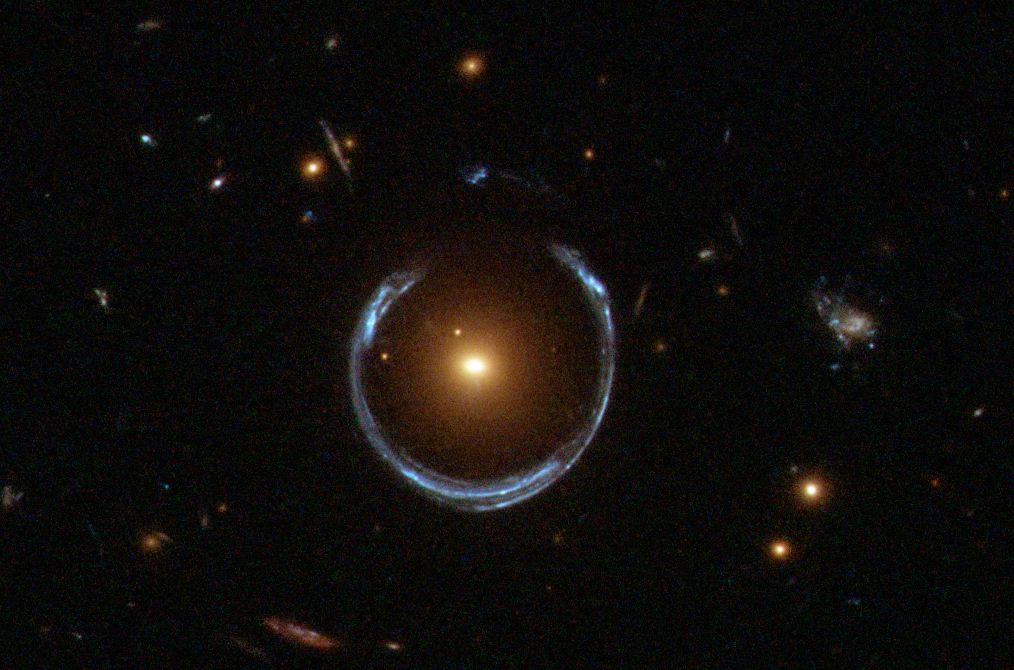
\includegraphics[width=0.4\textwidth]{einstein_ring}
   \label{fig:einring}
   }
   \qquad
   \subfloat[Einstein's cross]{
   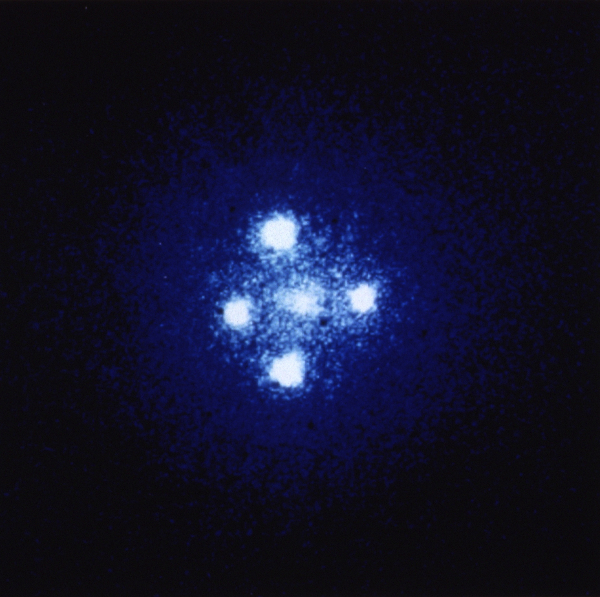
\includegraphics[width=0.4\textwidth]{einstein_cross}
   \label{fig:einsteincross}
   }
   \caption{Two examples of strong lensing effects. a) shows light from
   a distant blue galaxy being distorted by the central galaxy LRG 3-757
   \cite{einsteinring}. b) shows four images of a distant quasar being lensed by a
   foreground galaxy \cite{eincross}.}
   \label{fig:stronglens}
   \end{figure}
\subsection{Poisson Processes}
\label{sec-2-2}

   There are many situations in which one can benefit from a good model of the
   number of events of interest that occur in a given period. Poisson processes
   are \emph{stochastic processes} that can be used to do create such models. A
   stochastic process is a way of representing the evolution of a random value
   or system over time by using collections of random variables. Most such
   processes do not evolve in a \emph{deterministic} way. That is, the way they
   change as time passes is not predictable. Poisson processes are part of a
   family of stochastic processes which count the number of events and their
   time of occurrence in a given interval. They have been used to model the
   number of incoming requests to a server \cite{arlitt1997internet}, the number
   of calls made to emergency services \cite{hajjam2008approach}, and the rate
   of radioactive decay \cite{cannizzaro1978results}. In their basic form,
   Poisson processes have the following important properties
   \cite{ross1997simulation}:
\begin{enumerate}
\item $N(0)=0$.
\begin{itemize}
\item $N(t)$ represents the total number of events that occurred up until time
     $t$. Thus, if $N(0)=0$, it follows that the process begins at $t=0$.
\end{itemize}
\item The numbers of events occurring in disjoint time intervals are independent.
\begin{itemize}
\item The \emph{independent increment} assumption. This states that $N(t)$, the
     number of events that occur up to time $t$ is \emph{independent} of the
     number $N(t+s)-N(t)$, i.e. the number of events in the time interval
     between $t$ and $s$. In other words, the number of events that occur in one
     interval does not have an effect on the number of events in any other time
     interval.
\end{itemize}
\item The probability distribution of the number of events that occur in a given
   interval is dependent only on the length of the interval.
\begin{itemize}
\item The \emph{stationary increment} assumption. The implication of this is that
     the probability distribution of $N(t+s)-N(t)$ is the same for all values of
     $t$. That is, the likelihood of $n$ events occurring in the above time
     interval does not change, regardless of the value of $t$.
\end{itemize}
\item No counted occurrences are simultaneous.
\begin{itemize}
\item For all events that occur in the duration of the process, no two events
     will occur at the same time.
\end{itemize}
\end{enumerate}

   Each Poisson processes is governed by a \emph{rate parameter}, $\lambda$,
   which represents the number of events that occur in each time interval. As we
   are counting events, it is clear that the rate parameter can never go below
   zero---there cannot be a negative number of events in a given time
   interval. There are two types of Poisson processes, \emph{homogeneous} and
   \emph{non-homogeneous}. In a homogeneous Poisson process (HPP), the rate
   parameter is constant for the entirety of the process. This means that in
   every interval, the same number of events are likely to occur. In contrast, a
   non-homogeneous Poisson process (NHPP) has a rate parameter which
   varies. This means that the rate at which events occur varies as the process
   continues. As such, the value of $\lambda$ becomes a function of time,
   written as $\lambda(t)$. As a result, the stationary increment assumption
   does not apply to NHPPs. Figure \ref{fig:poisson} shows some examples of how
   the Poisson process evolves over time.
   \begin{figure}
   \subfloat[Homogeneous]{
   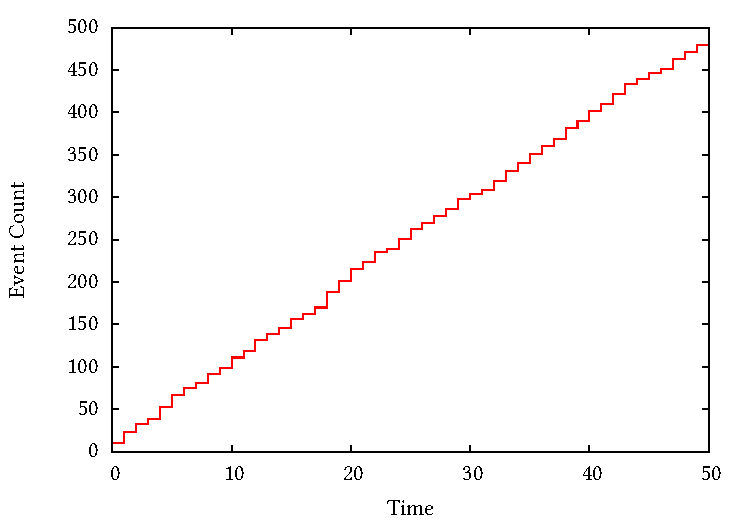
\includegraphics[width=0.5\textwidth]{homplot}
   }
   \subfloat[Non-homogeneous]{
   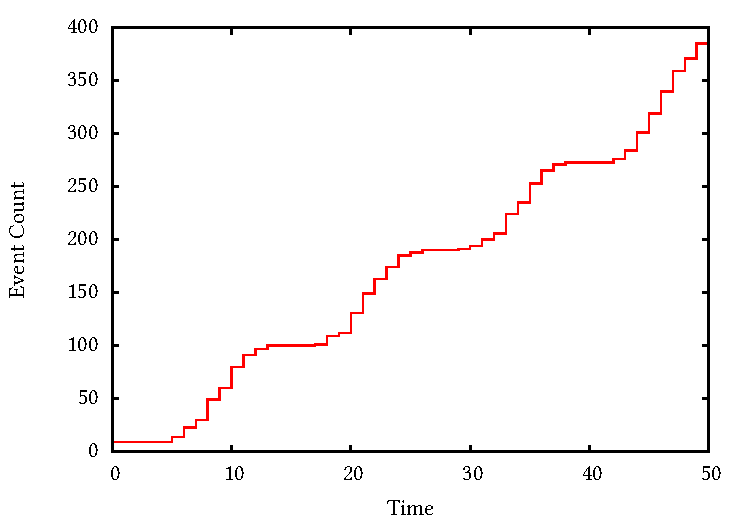
\includegraphics[width=0.5\textwidth]{nonhomplot}
   }
   \caption{Two examples of Poisson process paths. The homogeneous process has a
   rate parameter $\lambda=$ 10, and the non-homogeneous rate parameter varies
   depending on the value of a sine function.}
   \label{fig:poisson}
   \end{figure}
\subsection{Regression}
\label{sec-2-3}

   Regression is a statistical technique used to fit lines or curves to data
   points in order to find some sort of relationship between them. The number of
   variables in the data is important. One of the variables is called a \emph{dependent}
   variable. We want to find the relationship between this variable and the other
   variables, called \emph{independent} variables. What makes one variable
   dependent and another independent? Consider the expression $y=f(x)$. If $f(x)$
   is some function of the variable $x$, then we know that the value of $y$ depends
   on the value of $x$. This is where the names come from. In this simple example,
   $x$ is the independent variable, and $y$ is the dependent variable. There can be
   multiple independent variables, but only a single dependent variable.

   Linear regression is used in many different fields to find the trend between
   variables. It is heavily used in economics to make predictions about what
   happens in many economical situations. Finding trends in data is useful to many
   people in different ways.
\begin{itemize}
\item example of residuals. Show two linear estimates with the residuals sketched,
  one with a better fit than the other.
\end{itemize}
\subsection{Kernel Density Estimation}
\label{sec-2-4}

   This is another method which can be used to estimate functions, but which
   applies specifically to the probability density function of random
   variables. This technique uses \emph{kernels} to estimate the function
   densities. A kernel is a function which has some parameters. To estimate
   functions, kernels are centred at certain points along the axis which is being
   estimated. The spread can be either at uniform intervals, each sample value,
   etc. Kernels may have a weight assigned to them. Varying the parameters of
   the kernels results in different properties of the estimate. There are many
   different kernels that can be used. Different kernels are used in different
   applications.
\begin{itemize}
\item Show some examples of different kernels
   \begin{center}
   \begin{figure}
   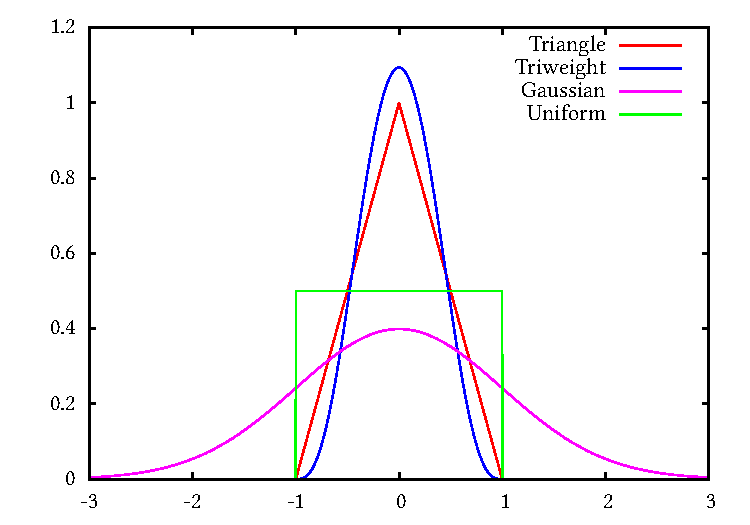
\includegraphics{kernel}
   \caption{Some examples of kernels commonly used for kernel density estimation.}
   \label{fig:kern}
   \end{figure}
   \end{center}
\end{itemize}
\section{System}
\label{sec-3}

  In this section we provide an overview of the system, and explain some of the
  details behind parts of the system which do not warrant their own sections in
  the report. We also give some idea about the design decisions used in the
  implementation. Discussion of the programming methodologies and ideas used can
  be found in the \ref{sec-4} section. The system is very large (over 7000 lines
  of C code), and we therefore attempt to detail the general ideas behind each
  part of the implementation rather than an in depth discussion of the
  techniques. Each subsystem described in sections \ref{sec-5}--\ref{sec-7} also has its own section describing some of the
  important parts of its implementation.
\subsection{Design}
\label{sec-3-1}

   When designing the system, we made the decision to split the three main
   pieces of required functionality into two groups. The generation of streams
   and functions would make up one subsystem, and the function and time delay
   estimation would make up another. This division is logical, as both of these
   subsystems perform two completely different tasks. They are only linked by
   the fact that the generators produce data that can be used by the estimators,
   but it is not strictly necessary for the data to come from inside the
   system---as long as it has the structure required by the estimators it can be
   used. However, since in our case the two subsystems are part of the same
   system, we need to be able to run them both from the same executable, and to
   do so we simply link them by allowing the subsystem which is to be run to be
   selected. Figure \ref{fig:sysstruct} gives an overview of the structure of
   the system.

   As with any large program, there will inevitably be some code which has to be
   used in different places in the program. We could just write the code twice,
   but this is very bad practice, and leads to more difficulty in both checking
   that the system works correctly, and modifying it later. Instead of allowing
   this to happen, code that might need to be used more than once is put into
   libraries which are shared between all subsystems.

   The input and output of the system is another important thing that must be
   considered. The system should be able to read data which follows some sort of
   structure. However, the structure should be simple so that data from as many
   sources as possible can be read in with minimal effort on the part of the
   user. If data has to be converted into some strange format before it can be
   read, then this is clearly sub-optimal. As such, the input to the system is
   from simple text files, which are easy to construct, and easy to read
   in. Output from the system, both in terms of output to the interface, and
   also output files, also need to have some meaningful structure, and the
   results of calculations should be clear. Output files should not contain any
   unneeded information. However, the needs of users is different. Sometimes
   more data will be required, and sometimes no output files are required at
   all. To deal with these cases, there needs to be some way to define how
   verbose output should be.

   For user interaction to occur, there needs to be an interface between the
   program and the user. In our case, the need for user interaction is
   relatively minimal. Once parameters are set, the program does not need any
   other input from the user. Results are mostly numbers and graphs. Textual
   output is simple to display, and there are many utility programs that can
   parse data files to draw graphs. As such, we decided not to use a command
   line interface over a graphical one. The development of a graphical interface
   is time consuming, and requires a lot of thought to be put into design. On
   the other hand, interaction with the command line is simply a question of
   reading text responses or parsing parameters. A graphical interface for the
   system would provide little benefit to the user in terms of additional
   information. There are some issues from the usability perspective, but the
   target audience for this program is not the average user. Most scientists
   interact regularly with computers, and astronomers in particular often use
   computer-based data processing tools. The system is a tool to use for data
   processing, not something that requires constant interaction with the
   user.

   Finally, in order to test the various methods developed, there has to be a
   way of running controlled experiments on the system. For this purpose, a
   wrapper around the estimator subsystem which can execute that subsystem
   multiple times with controlled parameters is a necessity.

\begin{itemize}
\item scripts?
\item structured filenames
   \begin{figure}
   \centering
   \pgfdeclarelayer{background}
   \pgfdeclarelayer{foreground}
   \pgfsetlayers{background,main,foreground}
   % horizontal separation
   \def \hnsep {0.5}
   \tikzstyle{sub}=[draw, fill=blue!20, text width=5em, 
   text centered, minimum height=2.5em, node distance=1.5cm]

   \begin{tikzpicture}
   \node (param) at (2,3) [sub] {Parameter file};
   % libs group
   \node (lib) at (6,3) [sub] {Libraries};
   % generator group
   \node (gen) at (2,0) [sub] {Generators};
   \node (strout) [sub, below of=gen] {Stream Data};
   % estimator group
   \node (est) at (6,0) [sub] {Estimators};
   \node (estout) [sub, below of=est] {Estimator Output};
   % experimenter
   \node (expparam) at (10,3) [sub] {Experiment Parameters};
   \node (explbl) at (10,0) [sub] {Experiment};
   \node (expout) [sub, below of=explbl] {Experiment Results};
   % launcher
   \node (launcher) at (0,1.5) [sub] {Launcher};
   % Draw the rest on the background layer
   \begin{pgfonlayer}{background}

   % path from expparam to experiments
   \coordinate [above=0.5 of explbl] (expln) {};
   \coordinate [below=0.8 of expparam] (exppjoin) {};
   \draw [line width=1pt] (expparam.south) -| (exppjoin);
   % path from experiments to exp out
   \draw [dashed,->,line width=1pt] (explbl.south) -- (expout.north);

   % launcher arrows
   \path (est.north)+(-0.3,-0.13) node (estla) {};
   \draw [->,line width=1pt,red] (launcher.east) -| (estla);
   \path (gen.north)+(-0.3,-0.13) node (genla) {};
   \draw [->,line width=1pt,red] (launcher.east) -| (genla);
   \path (explbl.north)+(-0.3,-0.13) node (expla) {};
   \draw [->,line width=1pt,red] (launcher.east) -| (expla);

   % library arrows
   \path (est.north) node (esttop){};    
   \coordinate [above of=gen] (gentop) {};
   \coordinate [below=0.8 of lib] (lsplit) {};
   \draw [-,line width=1pt] (lib.south) -- (lsplit);
   \draw [->,line width=1pt] (lsplit) -- (est.north);
   \draw [->,line width=1pt] (lsplit) -| (explbl.north);
   \draw [->,line width=1pt] (lsplit) -| (gen.north);

   % path from param to library link
   \coordinate [above=0.5 of lsplit] (tt) {};
   \coordinate [right=0.5 of param.east] (pright) {};
   \draw [line width=1pt] (param.east) -- (pright);
   \draw [line width=1pt] (pright) |- (tt);

   % estimator arrows
   \draw [dashed,->,line width=1pt] (est.south)--(estout.north);
   \coordinate [right=0.9 of estout] (restout) {};
   \coordinate [above=0.5 of explbl] (abvexp) {};
   \draw [line width=1pt] (estout.east) -- (restout);
   \draw [line width=1pt] (restout) |- (abvexp);

   % generator arrows
   \coordinate [above=0.5 of est] (abvln) {}; %above length est
   \coordinate [right=0.9 of strout] (rstrout) {};
   \draw [dashed,->,line width=1pt] (gen.south) -- (strout);
   \draw [line width=1pt] (strout.east) -- (rstrout);
   \draw [line width=1pt] (rstrout) |- (abvln);

   \end{pgfonlayer}
   \end{tikzpicture}
   \caption{A simplified overview of the system structure. Solid lines indicate
   the dependencies of a given subsystem, and Dashed lines indicate output from a
   subsystem. The red lines indicate what the user can access through the launcher.}
   \label{fig:sysstruct}
   \end{figure}
\end{itemize}
\subsection{Parameter Files}
\label{sec-3-2}

   The parameter files are used to configure the settings of all parameters that
   affect the functioning of the system. Separate files are used to configure the
   estimators and generators, and the experimenter. The syntax is very simple; the
   \texttt{\#} symbol defines a comment, and that line will be ignored when the
   file is parsed. A parameter is defined as an string of ASCII characters followed
   by a single space, followed by more ASCII characters. Each file is split into
   several sections, to aid the user in finding the parameters they are looking
   for. All parameters have comments describing their effect on the behaviour of
   the system, what values they can take, and other information relevant to the
   user. As the parameter files are quite long and require specific parameters to
   be present, functionality for generating parameter files with default settings
   are provided.
\subsubsection{System File}
\label{sec-3-2-1}

    The most used parameter file is the one which controls the behaviour of the
    estimators and generators. This file allows the setting of output filenames,
    generation parameters for the stream generator, including the interval length,
    start time, and the expression used to generate the streams. The random function
    generator can be set up to change the multiplier applied to the Gaussians,
    change their resolution, and define how the standard deviation is set. The
    configuration of all the parameters used by estimators is also done here. Time
    delay estimator behaviour is also determined by the settings in this
    file. The sections describing the implementation of parts of the system explain
    the exact parameters used and how they affect the behaviour.
\subsubsection{Experiment File}
\label{sec-3-2-2}

    The experiment parameter file is separate from the system parameter file as it
    may be desirable to use different parameter files for the same experiment. The
    experiment file contains parameters which affects the naming of output files,
    and allows the configuration of the intervals in which data is withheld in model
    selection. The most important parameters are those which define the names and
    parameters to test during the experiments.
\subsection{Libraries}
\label{sec-3-3}

   Each part of the system makes extensive use of custom libraries. Each library
   consists of a header file which contains the function prototypes and include
   information, along with a separate file for the functions, which are compiled by
   \texttt{libtool} into a convenience library. The advantage of using
   \texttt{libtool} over other ways of constructing libraries is that it can create
   both shared and static libraries. This means that if the library needs to be
   re-used elsewhere it is simple to take the shared object file created and
   compile the program including the library by passing the standard
   \texttt{-l[libname]} syntax to \texttt{gcc}. Since the libraries contain various
   functions which are useful not only for this system, this is a useful feature to
   have as the libraries can be easily re-used. Due to some interdependencies,
   between the lower level convenience libraries, they are merged into one main
   library, again functionality provided by \texttt{libtool}. The main function of
   the libraries is to abstract out code which may be used multiple times in order
   to reduce clutter, and avoid code duplication and the increased likelihood of
   errors associated with it. 
\subsubsection{Parameter List}
\label{sec-3-3-1}

    The parameter list library defines a singly-linked list which is used to
    store data parsed from the parameter files which contain parameters that
    modify the behaviour of the system. The functionality implemented by this
    library is very important, as almost all functions outside the libraries
    require one of these lists to perform their tasks. The library provides the
    functions for adding elements to the list and finding its length. A function
    for removal of elements is not provided, as there is no situation which
    should necessitate the removal of elements from the list. There is also
    functionality for checking whether a parameter with a given name exists,
    retrieving the value of a parameter, and setting the value of a parameter.

    There are multiple retrieval functions, each of which retrieves values of
    different types. The parameter list is constructed in such a way that all
    values in it are stored as character arrays. This means that if a parameter
    value is required by some function, it must be converted into the type which
    that function requires. Since it is known inside the function which type is
    required, the relevant function can be called. Functions to read
    \texttt{double} and \texttt{int} types are provided, along with a function
    to retrieve the character array. In addition, some of the parameters in the
    files are comma-separated lists of integers or doubles, which must be parsed
    into arrays before they can be used. The parsing also applies to the
    \texttt{double} and \texttt{int} types, which must be converted from string
    form into the correct type. In order to reduce code duplication, the
    conversion of the variables is done inside the retrieval function.

    The issue of whether the parameters should be parsed into the correct types
    upon reading of the file may be raised, but we believe that this solution is
    more appropriate. Firstly, it is often the case that not all parameters
    present in the file are required when any given task is executed by the
    system. Therefore, parsing all the parameters upon read may be a waste of
    processing time. In addition, having to parse parameters requires knowledge
    about what types they should be. This can be deduced within the code, but
    would require more complex logic. The storage would also be complicated by
    this, as the list would be required to store variables of multiple types. As
    mentioned above, parsing parameter values only when they are needed, and in
    contexts where their type is known means that the current structure performs
    its role well.
\subsubsection{Mathematics}
\label{sec-3-3-2}

    As the name implies, the mathematics library provides the mathematical
    functions required by the system which are not provided by the standard C
    library. Some of the library functions are based on functionality provided
    by the GNU Scientific Library \cite{gsl}, particularly those which calculate
    probability density functions or require random number generators. The most
    important part of the library is the functionality it provides for
    computations to do with Gaussians, in particular the discrete Gaussian
    transform. It also provides some basic useful functions, such as finding the
    minimum and maximum values in arrays, averaging, summing, adding to or
    multiplying arrays, and some implementations of statistical functions such
    as the root mean square error, standard deviation and the like. Functions
    which are critical to the operation of the system will be described in the
    implementation section of the relevant subsystems.

    The most challenging part of the implementation of the library was to get
    around the issues caused by double precision values. Functions which deal
    with calculations based on timings require a certain precision on the start
    and end times of intervals to work correctly. Due to the nature of their
    implementation, calculations with doubles often result in numbers which are
    only very close to the actual value. Particular problems were encountered
    when incrementing a value by a floating point number and comparing it to
    another. The floating point increments caused the value to be slightly (on
    the order of \num{1.0e-20}) below the actual value, and this caused
    calculations to be incorrect and resulted in a cascade of erroneous
    calculations. To deal with this problem, functions for comparing doubles to
    a specific precision were implemented.
\subsubsection{Input/Output Utilities}
\label{sec-3-3-3}

    This library implements functionality for reading from and outputting to
    files, as well as for checking the state of files and directories on the
    system. It is also used to parse the parameter file into the system, and as
    such defines the syntax that the parameter file must follow. We were unable
    to find a library which provided similar functionality to the Java
    Properties class, which allows the structured reading and storage of
    parameters, and so implemented a simplified version in the form of the
    parameter files. This library also reads in event data files, which are
    needed as input to the estimators, and can retrieve either all events, or
    data in a specific interval.

    As well as reading in data, the library also serves to output data from
    various data structures used within the system. This ranges from simple
    arrays to more complex data structures used to store representations of
    Gaussians or function estimates.
\subsubsection{General Utilities}
\label{sec-3-3-4}

    The final library is for functions which do not fit in anywhere else, such
    as memory allocation and freeing, printing structs and some error checking
    functions. There are also functions for generating default parameter
    files. The functionality of this library is relatively limited, but it means
    that the rest of the code in the system is much cleaner, as memory
    allocation and freeing of relatively complex structs can be done with a
    single function call. This abstraction of the memory management also makes
    dealing with the memory much easier---it is more difficult to make a mistake
    when freeing something, as the functions are already defined.
\subsection{External Libraries and Tools}
\label{sec-3-4}

   The system uses a number of external libraries to augment the C standard
   libraries, and to reduce the need for us to write code which has already been
   written elsewhere. The GNU Scientific Library \cite{gsl} provides the system
   with random number generators that can be used to provide more varied random
   numbers than the standard library provides, and also gives access to
   probability density function computations. The Check framework \cite{check}
   is used to implement automated tests for the system, and is part of the GNU
   build system, which provides assistance for making source code packages
   portable to many Unix systems. Our system makes use of the \texttt{automake}
   and \texttt{libtool} frameworks to generate shared library files and
   makefiles, and its structure outside the code follows that of the standard
   GNU package. The MuParser library \cite{muparser} is used to parse
   expressions used to generate stream data. The Valgrind framework was used to
   debug memory errors \cite{valgrind}.
\subsection{Interface}
\label{sec-3-5}

   User interaction with the system is done via a command line
   interface. Various flags passed to the executable change the behaviour of the
   system, but the majority of behaviour can also be controlled through the
   parameter file. The standard C libraries provide a useful function,
   \texttt{getopt}, specifically for the parsing of command line options. This
   function allows the parsing of short options, such as \texttt{-g}, or with
   the \texttt{getopt\_long} function, longer options such as
   \texttt{--generate} can be parsed. Users familiar with *NIX systems will no
   doubt recognise such options, as they are used in almost every program which
   can be run from the command line. The parsing of options is done by the
   launcher, which is the only part of the system that the user interacts with
   directly. Depending on the options received, the system behaves in a
   different way. Each subsystem can be called using a specific option, and
   checks are made to ensure that only a single subsystem is being called. When
   an error occurs in the parsing of options, which can arise due to an option
   with a required parameter not having anything passed to it, or as a result of
   multiple subsystem calls, an error message is printed informing the user of
   the error. As with many command line programs, instructions on what switches
   are available, and some information on what they do is available by using the
   \texttt{-h} or \texttt{--help} options. The help information is also printed
   when there is some issue when parsing the parameters. To better facilitate
   the addition and removal of options, the value of each option is stored as a
   flag in a struct which is then passed to another functions which uses its
   contents to take the user's desired route through the program logic. The
   launcher does only the minimum amount of work required to get the system to
   run. Once it has parsed the options, it calls the relevant subsystem and its
   job is done. Instructions on how to use the system can be found in Appendix
   \ref{sec-10-2}.
\subsection{Experimenter}
\label{sec-3-6}

   The purpose of the experimenter is to run the estimation subsystem multiple
   times, with different parameter settings. Its behaviour is modified by a
   separate parameter file. The code is designed in such a way that new
   experiments on different parameters can be added and removed with minimal
   effort on the part of the user. 

   A simple experiment can be set up by modifying just a few lines in a
   parameter file used to configure the behaviour of the experimenter. The
   experiment must be given a name, so that the system can reference it. Some
   parameters to experiment on must be set, and the type of estimator to use to
   estimate the function must also be specified. An additional parameter is used
   to specify whether an experiment with the given name should be run or not. To
   allow for greater flexibility, the parameter values to test can be defined as
   ranges. For example, entering \texttt{2,4,...,10} as the value for a
   parameter will result in values of 2, 4, 6, 8 and 10 being experimented
   on. There are two types of experiments that can be performed; the estimation
   of functions, or the estimation of the time delay. The ability to do
   experiments on these separately is important, as model selection must be
   performed to determine the optimal parameter settings for a given set of test
   data before experiments on the time delay can be done, and there are
   functions which can be used to do this. However, the system does not require
   model selection to run. Once streams of photons have been generated, the
   experimenter can be set to create a copy of those streams with the data in
   certain intervals removed.
   
   The next stage is to run the function estimators on these streams with
   different parameter combinations and see which combinations produce the best
   results. Parameter settings are co-varied, which means that all possible
   combinations of parameters are tested. All possible values of parameters are
   stored in separate arrays for each parameter, and each has a pointer which
   indicates which value of the parameter should be used by the estimator. After
   each run of the estimator with a given set of parameters on all test data has
   been completed, the index of the last parameter is incremented by 1, and the
   process is repeated. Once the value of the index exceeds the length of the
   array, it is reset to 0, and the index on the second to last parameter is
   incremented by 1, and this process continues until all indices return to 0. A
   system that works in a similar way is a milometer---once the digits column
   reaches 9, travelling a mile will reset that value to 0, and the value in the
   tens column will be incremented to 1, and this process continues until the
   value in all columns is 9, and with the next mile everything is reset
   to 0. After the experiment for a set of parameters is complete, the results
   of the estimates are analysed, and each is given a score based on a sum of
   log probabilities. The value of the function in each interval in which data
   was withheld is compared to the actual value. The closer the estimated and
   actual values are, the higher the score. Once all parameter combinations have
   been run, the best combination of parameters for each stream in the test data
   is written to file. Files are also produced in each sub-directory which give
   information about the parameters used for experiments in that directory. 

   Once the model selection is done, the optimum parameters can be extracted
   from the results and the time delay can be estimated. The time delay results
   are also processed, with the estimate and error for each stream pair, and the
   mean, standard deviation and mean error of a set of streams pairs being
   output to file. Functionality for running large numbers of experiments is
   provided by a number of shell scripts. Instructions on running experiments
   can be found in Appendix \ref{sec-10-3}.
\section{Development}
\label{sec-4}

  In this section, we discuss the programming methodologies and project management
  ideas used during the development of the project.
\subsection{Development Process}
\label{sec-4-1}

   The development process was made up of three key stages. First, before
   writing any code, the ideas behind the part of the system that was to be
   implemented were sketched out in a physical notebook. The details of this
   stage were specific to the needs of every bit of functionality, but generally
   consisted of the same decomposition of what was required. What parameters
   does it need? How does the input need to be processed? What should be output?
   For more complex parts of the system, we also planned out how it would
   connect to the main parts of the system, either in terms of data structures,
   or where it should be called from. When more complex algorithms had to be
   implemented, we wrote a prototype on paper and tested it for a few simple
   cases to check its correctness.

   Once we had a good idea of the structure of the code, we implemented a
   prototype which was loosely connected to the system. This prototype would
   have its own internal variables and would not actually return anything to the
   system, instead printing all its output to the terminal. The output was
   checked manually to verify its correctness. At this stage, automated tests
   were also written for many functions, particularly those which had an
   important role in mathematical calculations or error checking. By the end of
   this part of the process, we had a minimal working version of the function
   that we wanted to implement.

   The final stage was to integrate the function or subsystem fully with the
   main system, abstracting out all the internal function variables to the
   parameter files, or taking them in as parameters to the function. More
   rigorous error checking was also implemented at this stage to ensure the
   correctness of parameters. Once integrated, tests were run again to confirm
   that no bugs had been introduced by the conversion.
\subsection{Development Methodologies}
\label{sec-4-2}

   We used a few principles of software development that we believed could guide
   us to create a better system. The Unix philosophy of operating system
   development has many ideas that can be used to develop much smaller
   systems. In \emph{The Art of UNIX Programming}, Raymond abstracts some ideas
   behind the philosophy into a set of 17 short rules \cite{artunix}. We found
   that a subset of these rules were applicable to our system:

   \begin{description}
   \item[Rule of Least Surprise] In interface design, always do the least
   surprising thing.
   \item[Rule of Modularity] Write simple parts connected by clean interfaces.
   \item[Rule of Optimising] Prototype before polishing. Get it working before
   you optimise it.
   \end{description}
   
   Although the interface in our system involves minimal interaction, the rule
   of least surprise is still a good one to follow. When designing the behaviour
   of the launcher, we considered what the expected behaviour would be, and
   implemented functionality which made this behaviour possible. However minimal
   the interaction with a system is, it is still important to consider the
   expectations that a user may have. One particular example is the presence of
   a help command which gives information about what the program does and what
   options it can parse. Entering \texttt{ls --help} on a Linux system gives an
   example of the contents of such a printout. We ensured that this was present
   in our implementation of the launcher.

   Our system is not so large as to have properly defined interfaces, but the
   content of subsystems, and the links between them are vitally
   important. During our implementation, we tried to follow the rule of
   modularity by making each part of the system as simple as possible. The
   functions which execute a particular task should be grouped together, and any
   functions which are not a direct part of that process should be grouped
   elsewhere. For example, the functions which run the estimators are very
   short, and are grouped together in one file. The estimators themselves are
   separate entities---they are not grouped together in one large file which
   contains them all, but instead in their own dedicated file. Functions which
   are used by the baseline estimator, for example, are of no use to the
   iterative weighted least squares estimator, as their tasks are very
   different. Connections between parts are also made to be simple, by
   encapsulating data in structs and passing them around as necessary.

   As mentioned in the previous section, the rule of optimising was a key part
   of the development process. Moving from prototype to implementation to
   polishing means that time is not wasted optimising or trying to fix something
   that is fundamentally broken.

   In \emph{The Pragmatic Programmer}, Hunt and Thomas put forward their ``DRY''
   (\emph{D}on't \emph{R}epeat \emph{Y}ourself) principle, which states that
   ``Every piece of knowledge must have a single, unambiguous, authoritative
   representation in a system.'' We believe this to be the most important
   principle we have followed, as code duplication has many issues, mostly
   stemming from contradictions. The libraries are our attempt to ensure that
   there is one function for a single task, and the parameter files represent
   the single definition of control parameters in the system.
\subsection{Testing}
\label{sec-4-3}

   Any system requires testing to verify its correctness, and we have
   implemented a large number of tests for those functions which are central to
   the correct functioning of the system. Some functions, such as those which
   perform the estimation, it is not feasible to check, as the actual results
   that should be obtained for a normal input are not easily calculated without
   relying on the system itself. In cases where it is possible, we have
   concentrated on those functions which consist of more than just simple
   statements. Those functions which perform mathematical computations and error
   checking are the ones which have undergone the most rigorous checks.

   A total of 62 tests have been implemented, each of which contain multiple
   cases to check edge cases. Of these, 56 check library functions. Checks on
   functions in the mathematics library make up over half of those.

   Tests are implemented using the Check framework \cite{check}, which is a unit
   testing framework designed for the C language. The main reason for its use is
   its integration into the GNU Autotools framework, which is used for automatic
   configuration and compilation of the code.
\subsection{Version Control}
\label{sec-4-4}

   The project was kept under version control using the \texttt{Git} and
   \texttt{SVN} revision control systems. The Git repository was used as the
   main repository, with all commits being made there. The SVN repository was
   used as a backup, with tagged versions being committed to that for backup
   purposes.

   A branching strategy was chosen, in an attempt to bring the project closer to
   one which might be performed in an industry environment. Several searches for
   a branching strategy led us to use one proposed by Driessen
   \cite{driessen}. In this strategy, there are two main branches,
   \texttt{master} and \texttt{develop}. The state of \texttt{master} reflects
   the current version, and \texttt{develop} reflects the current state of
   development. There are three supporting branches, which deal with features,
   hotfixes and releases. In our case, dealing with hotfixes was not important
   as we were not releasing production software. For each new feature, or large
   change that was made to the system, we moved development to a new branch so
   as not to impact the main development branch. Branches were merged back to
   the main development branch when the feature was complete. When a large
   milestone in the project was completed, such as the completion of a
   subsystem, we branched into a separate branch for that release to make some
   modifications to information about the code, and then merged the release
   branch with \texttt{master} and \texttt{develop}.

   Commits were made to the development branch when a small feature was
   completed, or some modifications were made. With this sort of regular commit
   activity, it would be easy to revert to a working version should a bug be
   found, and attempt to locate the root of the problem.
\subsection{Project Management}
\label{sec-4-5}

   As mentioned above, we kept detailed notes of algorithm prototypes and ideas
   about how to proceed with the implementation of the project in a physical
   notebook. This notebook also served the purpose of detailing mathematics and
   ideas that were relevant to the project, and how they might be used. 

   In addition to the notebook, we kept a change log of all the modifications
   made to the code in a text file which was updated with every commit to the
   repository. In this log we detailed which parts of the code were changed,
   what change was made, and if relevant, the reasoning behind the change. Not
   only the change log, but also each individual commit to the repository went
   into a reasonable amount of detail about the changes that were made. With
   this log, it is easy to go back in the time line of the development of the
   system and see exactly when and why a specific change was made, in a much
   more accessible form than physical writing. 
\section{Simulation of Photon Streams}
\label{sec-5}

  The first step in building the system was the development of a photon stream
  simulator. The ability to simulate photon streams means that the system can be
  tested on many different stream types, so that we are able to determine where
  its strengths and weaknesses lie. While many simulation tools are very complex,
  our system does not require simulation of the source objects or the movement of
  photons, as we are only interested in their arrival time. A source can be
  represented by some random variable $X$, which indicates the variability of the
  source with time. Different types of sources will have different types of
  characteristic functions---the variation in a quasar will be very different to
  that of an individual star, for example. A NHPP is an ideal way to represent
  this type of system. The function $\lambda(t)$ will represent the random
  variable, and the values output from the process will represent the arrival
  times of the photons. $\lambda(t)$ describes the variability of the source in
  time. In other words, it provides a rate parameter at each time $t$ for the
  duration of the simulation. To be able to simulate a wide variety of functions,
  it is necessary to have the capacity to generate functions with different
  characteristics.
\subsection{Function Generation}
\label{sec-5-1}

   To evaluate the performance of the function and time delay estimators, it will
   be necessary to test the accuracy of the estimates on different types of
   functions. To this end, the capability of generating random functions will be
   very useful. To generate random functions, we make use of \textbf{Gaussian
   kernels or just Gaussians?}. The generation process involves four simple steps:
\begin{enumerate}
\item Pick some value $\Delta t$ which represents the distance between the mean
   $\mu$ of successive Gaussians.
\item Define some value $\alpha$, where the standard deviation $\sigma$ of each
   Gaussian is determined by $\alpha\cdot\Delta t$.
\item For each Gaussian, choose some weight $w_i$, from a uniform distribution
   between -1 and 1.
\item Using some step $s$, sum all the Gaussians at each point on the $x$-axis which
   we get from these $s$ values.
\end{enumerate}

   The first step defines how spread out the Gaussians should be in the interval
   $[t_0, T]$ in which the function is to be generated. If the spread is large,
   then depending on the standard deviation of the Gaussians there will be many
   points on the interval where the value of the function is zero. On the other
   hand, with a low value of $\Delta t$, most points on the line should have some
   non-zero value.

   The $\alpha$ parameter determines the standard deviation $\sigma$ of all the Gaussians
   used to generate the function. The value of $\sigma$ is the one that affects the
   final function the most. Low values will result in each Gaussian covering only a
   small interval, so if the Gaussians are sufficiently spread out, the variation
   in the function will be much larger than if higher values of $\sigma$ are used.

   With just the above two steps, the functions generated would be very
   homogeneous, because each Gaussian has the same weight. With uniform Gaussians,
   there would be hills at each point where a Gaussian is centred, and very little
   to speak of in between, and the height of the function would never exceed a
   certain value. To introduce more variation, a weight $w_i$ is sampled uniformly
   from ($w_i \sim U(-1,1)$). Uniform sampling simply means that each value between
   -1 and 1 has an equal probability of being chosen. To further increase the
   variation in the functions that can be generated, some multiplier can be used,
   which scales the values of the weights, meaning that the function will have
   larger values over the whole interval.

   The final step is to calculate the values which will make up the
   function. Starting at the beginning of the interval $t_0$, we sum the values of
   all the Gaussians at points along the line until the end of the interval $T$ is
   reached. The points that are sampled are defined by $t_i=t_{i-1}+s$, where $s$
   is some sample step. The use of smaller sample steps results in a higher
   resolution. The sum of the Gaussians at time $t$ can be calculated by
   \begin{align}
   f(t) = \sum_{g\in G}w_g\cdot e^{-(t-\mu_g)^2/2\sigma_g^2}
   \end{align}
   Where $G$ is the set of Gaussians which make up the function, and $w_g$, $\mu_g$
   and $\sigma_g$ are the weight, mean and standard deviation respectively of the
   current Gaussian being processed.

\begin{itemize}
\item random functions using gaussian sums
\item explain how the gaussians are placed, how the standard deviation is
  calculated, what effect this has on the function shape
  ($\sigma=\alpha\cdot\Delta t$)
\item examples at various alpha and delta t values?
\item $w_t\cdot e^\frac{{x-\mu}^2}{2\sigma^2}$
\end{itemize}

   In addition to the random function generation, it may sometimes be useful to
   generate a function from a known expression, and the system includes this
   functionality as well, which will be described below.
\subsection{Generating Streams from Functions}
\label{sec-5-2}

   Once the function has been generated, we can use it to generate values for
   the random variable $X$ which governs a NHPP. To generate a NHPP, it is
   necessary to build on the generation of a HPP. It is well known that
   probability of an event occurring follows an exponential distribution. The
   rate parameter $\lambda$ determines how many events occur in a given time
   interval. Knowing this, we can calculate the time of the next event by
   sampling from this distribution. Generate a random value $U\sim U(0,1)$. The
   time $t$ to the next event is defined by
   \begin{align}\label{eq:homlambda}
   t=\frac{1}{\lambda}\log(U)
   \end{align}
   Using this calculation, it is possible to generate a realisation of a HPP for
   any length of time. This provides a base which can be extended to generate
   events from NHPPs. To generate events from the NHPP, we use a technique
   called thinning. The basic concept behind thinning is to generate a large
   amount of values, and then remove them based on some method. In the case of
   the NHPP, we generate events with a rate parameter $\lambda$, where
   $\lambda>\lambda(t)$ for $0<=t<=T$. In other words, the homogeneous lambda
   value must be larger than the value of the function we are generating from at
   any point. First, two random values are independently sampled from a uniform
   distribution between 0 and 1, $U_1,U_2\sim U(0,1)$. $U_1$ is used in
   \eqref{eq:homlambda} to find the next event time from the homogeneous process
   governed by $\lambda$. Using the time $t$ generated from that, the value of
   $\lambda(t)$ is found. Depending on the ratio between $\lambda(t)$ and
   $\lambda$, the event is kept or discarded. When the value of $\lambda(t)$ is
   close to that of $\lambda$, more events are kept because
   $U_2\leq\frac{\lambda(t)}{\lambda}$ will be true more of the time. The
   variation of $\lambda(t)$ in time means that events are generated
   proportional to the value of lambda.

\begin{itemize}
\item Need to generate event times - use Poisson process
\item start with homogeneous
\item extend homogeneous to non-homogeneous (explain math)
\item Issues with the implementation - must have $\lambda>\lambda(t)$ for all
  $0<=t<=T$.
\item Diagram showing HPP and NHPP
\item \href{http://preshing.com/20111007/how-to-generate-random-timings-for-a-poisson-process}{http://preshing.com/20111007/how-to-generate-random-timings-for-a-poisson-process}
\end{itemize}
\subsection{Implementation}
\label{sec-5-3}

   The function and stream generation functions form the \emph{generator}
   subsystem. The two different function generation methods use fundamentally
   different methods to generate functions. The random functions use Gaussians,
   which are represented in a struct containing the mean, standard deviation and
   weight of the Gaussian. We use another struct to store an array of Gaussians
   which represent the whole function. When one of these arrays is generated,
   its constituent Gaussians are output to a file so they can be used later if
   necessary. Once one of these sets of Gaussians is generated, it is passed to
   a function which implements the thinning procedure. To generate the $\lambda(t)$
   values, the sum of Gaussians in the generated array at the given time is
   used. A two dimensional array is returned, containing the time of each event,
   and the value of $\lambda$ at each time. Once the stream has been generated,
   depending on the requested output verbosity, the data is output to file. This
   process is repeated for the requested number of streams. Multiple different
   functions can be generated with one function call. Alternatively, a single
   function can be used to generate multiple stream pairs.

   The generation of functions using expressions is done in a very similar way
   to the Gaussian generation, but since an expression is being used there is no
   need to store the representation of the function in a special way. Events are
   generated and thinned using a very similar function to the Gaussian, but
   instead of an array take a \texttt{muparser} struct pointer which can be used
   to get function values out of the expression that has been parsed into
   it. This pointer is created in the setup function which reads data from the
   parameter file and parses the expression. If there is a syntax error in the
   expression, the program prints the location of the error using
   \texttt{muparser} functions and exits.

   The generation in both cases is split into several stages. In the first
   stage, the parameters required by the function are read from the parameter
   list. If there are parameters that have been passed in as options to the
   command line, they take precedence. Once these parameters are checked, the
   top level function makes multiple calls to the second function, depending on
   how many functions are to be generated. The job of the second level function
   is to make calls to the function which actually performs stream generation,
   and output the resulting data to file.

   This three-level structure is used throughout the system to separate the
   parameter retrieval and checking from the execution of the logic. This also
   means that if parameters have already been parsed and checked in another
   function, the second-level function can be called to get back the desired
   results.

   The configurable parameters for the generation functions include the value
   of $\Delta$ for each stream, the start time and length of the interval, the
   value of the homogeneous $\lambda$ to use in the thinning procedure, and the
   expression to use to generate the function. In the case of the Gaussian
   generator, the distance between Gaussians, the sample resolution and the
   weight multiplier can be specified. In addition, the standard deviation can
   be set to be calculated using $\alpha\cdot\Delta t$, or simply taken from a
   specified value.
\section{Function Estimation}
\label{sec-6}
\subsection{Baseline Estimation}
\label{sec-6-1}

   In this section, we present the baseline method for function estimation. The
   core of the estimator is based on the iterative weighted least squares estimator
   derived by Massey et.al \cite{massey1996estimating}, and in the next two
   sections we attempt to explain its derivation in simpler terms than in the
   original paper. The subsequent sections detail our additions to the simple
   estimators in order to form the final baseline estimator which will be used as
   the first of our function estimation methods.
\subsubsection{Ordinary Least Squares}
\label{sec-6-1-1}

    The ordinary least squares (OLS) estimator forms the core of the baseline
    estimator. This estimator will form an estimate by minimising the sum of squared
    residuals. It is important to note the difference between errors and
    residuals. In statistical terms, an \emph{error} is ``The difference between the
    observed value of an index and its ``true'' value'' \cite{2008oecd}, and a
    \emph{residual} is ``The difference between the observed value of a response
    variable and the value predicted by some model of interest''
    \cite{everitt2010cambridge}. The ``true'' in the definition of error is in
    inverted commas due to the fact that the true value of the function is
    unobservable---it is only possible to obtain a statistical sample. The residual,
    on the other hand, is the difference of the observation from some
    \emph{estimate} of the function. This first estimator estimates a linear
    function of the form $y=ax+b$, or a straight line. While this is not directly
    useful for estimating characteristic functions, it was developed in order to
    gain a deeper understanding of the ideas behind regression, and in order to
    construct a simple estimator which could then be extended.

    In order to estimate the function, the stream of events must first be converted
    into a form which is suitable for processing. To do this, we first pick a time
    interval $(0,T]$, and divide it into $N$ sub-intervals, or \emph{bins}. According
    to \cite{massey1996estimating}, the $k\text{th}$ bin $I_k$ is
    calculated by
    \begin{align}
    I_k&=\left(\frac{(k-1)T}{N}, \frac{kT}{N}\right],\,1\leq k\leq N
    \intertext{and the midpoint $x_k$ of each bin is}
    x_k&=\left(k-\frac{1}{2}\right)\frac{T}{N},\,1\leq k\leq N
    \end{align}
    Due to the independent increments property of Poisson processes, splitting the
    interval leaves us with $N$ bins, each of is defined by an independent Poisson
    random variable \cite{massey1996estimating} $Y_k$ with mean
    \begin{equation}\label{eq:lam}
    {\lambda}_k=\frac{T}{N}(a+bx_k)
    \end{equation}
    where $T/N$ is used to normalise the value of ${\lambda}_k$. The value of $Y_k$ in our
    case is the number of photon arrival times for each bin. In order to perform
    regression on the data, we need a model of the data. At this stage, we make the
    assumption that the data is represented by a linear function, so the model is
    linear. The model is used to connect the random variables and the parameters,
    and describes how they are related. Our model becomes $Y=\alpha+\beta x
    +\epsilon$, or $Y_k=\alpha+\beta x_k + {\epsilon}_k$
    \cite{massey1996estimating}. The values $\alpha$ and $\beta$ are the two
    regression parameters which we use to estimate the values of $a$ and $b$ of the
    characteristic function. \textcolor{red}{What is a regression parameter?}
    $\epsilon$ represents the Poisson error that is present in the data that we are
    trying to model. As mentioned before, this technique works by minimising the sum
    of squared residuals. The value of a residual can be computed by
    \cite{kenney1962mathematics}
    \begin{equation}\label{eq:residual}
    d_k=Y_k-(a+bx_k)
    \end{equation}
    However, since we cannot know the real values of $a$ and $b$, we must instead
    use the regression parameters $\alpha$ and $\beta$. Substituting these into
    \eqref{eq:residual} we get
    \begin{equation}
    d_k=Y_k-(\alpha+\beta x_k)
    \end{equation}
    With this, we can calculate residuals for our function estimate. This
    calculation by itself is not sufficient, though, as summing the residuals
    necessarily results in a value of zero \textcolor{red}{\textbf{FIND A CITATION FOR THIS!}}. To
    get a useful value from the residuals, we square the value of each residual.
    \begin{equation}\label{eq:sqres}
    d_k^2=(Y_k-[\alpha +\beta x_k])^2
    \end{equation}
    Until now, we have been ignoring ${\epsilon}_k$, the Poisson noise associated
    with the random variable. In order to compensate for this, it is necessary to
    introduce a weight $w_k$ for each interval, initialised to 1 as we are using
    the OLS technique \cite{massey1996estimating}. Introducing this weight into
    \eqref{eq:sqres} and summing over all bins, we have
    \begin{equation}
    \sum_{k=1}^N w_k(Y_k-[\alpha +\beta x_k])^2
    \end{equation}
    the residual sum of squares (RSS). We want to find the values of $\alpha$ and
    $\beta$ for which the RSS is minimised, and so the final expression becomes
    \begin{equation}
    \min_{\alpha,\beta}\sum_{k=1}^N w_k(Y_k-[\alpha +\beta x_k])^2
    \end{equation}
    which is known as the \emph{objective function}. Once the objective function is
    known, we can define estimators $\hat{\alpha}$ and $\hat{\beta}$, which we
    will use to estimate values of $\alpha$ and $\beta$ to find the minimum \cite{massey1996estimating}.
    \begin{equation}
    \hat{\beta}
    =\frac{\displaystyle\sum_{k=1}^N w_k(x_k-\bar{x})(Y_k-\bar{Y})}{\displaystyle \sum_{k=1}^N w_k(x_k-\bar{x})^2}
    =\frac{\displaystyle\sum_{k=1}^N w_k(x_k-\bar{x})Y_k}{\displaystyle\sum_{k=1}^N w_k(x_k-\bar{x})^2}
    \end{equation}

    \begin{equation}
    \hat{\alpha}=\bar{Y}-\hat{\beta}\bar{x}
    \end{equation}

    \begin{equation}
    \text{where}\quad
    \bar{x}=\frac{1}{N}\sum_{k=1}^N w_kx_k\quad \text{and}\quad
    \bar{Y}=\frac{1}{N}\sum_{k=1}^N w_kY_k
    \end{equation}

    If we ignore the effect of adding the weight $w_k$ for the time being, the
    calculation of $\hat{\beta}$ is equivalent to dividing the covariance of $x$
    with $Y$ by the variance of $x$ \cite{kenney1962mathematics}. This should allow
    us to understand more about how the value of the estimate changes depending on
    what the values of $x$ and $Y$ look like. The covariance is a measure of the
    strength of the correlation between two or more random variables
    \cite{covariance}. If high values of one variable occur when the other variable
    also has high values, then the covariance is positive. If high values of one
    variable occur when the other has low values, then it is negative. The variance,
    on the other hand, is a measure of the variation in values of a random
    variable. If all values are close to the mean, then the variance is small, and
    if there are large deviations from the mean value, then the variance is
    large. If the covariance is positive, then the values of $Y$ increase as $x$
    increases. The variance of $x$ depends only on the length of the
    interval---short intervals have low variance, and long intervals high
    variance. This is because the calculation of the variance is done by finding the
    distance to the midpoints of bins from the value of $\bar{x}$, which is the
    midpoint of the interval. It is clear that the sign of $\hat{\beta}$ depends on
    whether the covariance is positive or negative, and this in turn defines the
    sign of the gradient. The steepness of the gradient is defined by the magnitude
    of the covariance. Since the value of the variance is constant, the larger the
    magnitude of the covariance, the steeper the gradient. Once we know the gradient
    of the line, the calculation of the intercept is simple, so long as we know the
    value of a point on the line, and the point $(\bar{x},\bar{Y})$ is one such
    point. We rearrange the equation $\bar{Y}=\hat{\alpha}+\hat{\beta}\bar{x}$ to
    solve for $\hat{\alpha}$. Notice that since the values of $\bar{x}$ and
    $\bar{Y}$ do not change, the point defined by the mean values becomes a pivot
    for the line estimate. The addition of the weights adds bias into the calculation,
    taking into consideration the variation of those points which have a smaller
    estimated value of $\lambda$. The weight update calculation is discussed in the
    next section.

    We normalise the values of $\hat{\alpha}$ and $\hat{\beta}$ by multiplying the
    resulting estimate by the number of bins over the interval length. The fewer
    bins used in the estimate, the larger the bin count will be for each bin, and
    consequently the larger the estimated values will be. To return the estimate to
    the same scale, 
    \begin{equation}
    \hat{a}=\frac{N}{T}\hat{\alpha}\quad\text{and}\quad
    \hat{b}=\frac{N}{T}\hat{\beta}
    \end{equation}

\begin{itemize}
\item show non-normalised estimate vs normalised estimate
\end{itemize}

    As we are dealing with a Poisson process with a rate function, it is natural to
    impose a constraint on the values of $\hat{a}$ and $\hat{b}$ which states that
    the rate function must be non-negative throughout the entire interval $[0,T]$,
    since it is not possible to have a negative rate \cite{massey1996estimating}.
    \begin{equation}
    \hat{a}\geq 0\quad \text{and}\quad
    \hat{b}\geq -\hat{a}/T
    \end{equation}
    There are two cases in which this constraint can be violated; when $a<0$ or
    $b<-\hat{a}/T$ \cite{massey1996estimating}. In the first case, we set
    \begin{align}
    \begin{split}
    \hat{a}&=0\\
    \hat{b}&=\frac{N}{T}\frac{\displaystyle \sum_{k=1}^N w_kx_kY_k}{\displaystyle\sum_{k=1}^N w_kx_k^2}
    \end{split}
    \end{align}
    and in the second,
    \begin{align}
    \begin{split}
    \hat{a}&=-\hat{b}T\\
    \hat{b}&=-\frac{N}{T}\frac{\displaystyle \sum_{k=1}^N (T-x_k)Y_k}{\displaystyle \sum_{k=1}^N w_k(T-x_k)^2}
    \end{split}
    \end{align}
    \textcolor{red}{\textbf{Is this sufficient?}}
    Applying these adjustments in the cases in which the constraints are violated
    ensures that the final estimate is always within the required
    constraints. However, the adjustments introduce some non-linearity into the
    system \cite{massey1996estimating}. With this set of equations, the fundamental
    structure of the OLS estimator is complete. In the next section, we discuss the
    addition of weight update rules and finding estimates of $\lambda$.
\subsubsection{Iterative Weighted Least Squares}
\label{sec-6-1-2}

    \begin{figure}
    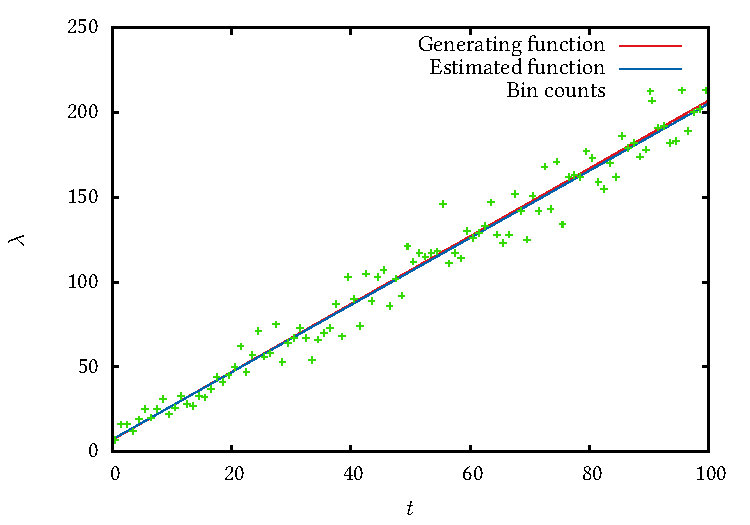
\includegraphics{lineest}
    \label{fig:line}
    \caption{IWLS estimate of a realisation of the function $y=a+bx$ where $a=$ 7
    and $b=$ 2.}
    \end{figure}
    The iterative weighted least squares (IWLS) estimator builds upon the OLS
    estimator. As the name suggests, the extension is to include an iterative
    part. The OLS estimator performs a single estimate of the function and leaves it
    at that. The IWLS estimator, on the other hand, repeats the process multiple
    times, updating its estimates. Perhaps the most important update to the
    estimator is the use of unequal weights, which change depending on the variances
    of the random variable which defines the bin which the weight is being applied
    to. A Poisson random variable has a variance that is equal to its mean---this
    means that a higher value of ${\lambda}_k$ results in a larger variance. To
    compensate for this, we give higher weights to bins which have lower values of
    $\lambda$, as the variances will be lower. As shown in equation \eqref{eq:lam},
    the value of $\lambda$ is easy to calculate, but the values of $a$ and $b$ must
    be known. In order to modify weights appropriately, we must be able to obtain
    estimates of $\lambda$, which can be done using \cite{massey1996estimating}
    \begin{align}
    \hat{\lambda}_k=\frac{T}{N}(\hat{a}+\hat{b}x_k)
    \end{align}
    The weights can then be updated using
    \begin{equation}
    \hat{w_k}=\frac{\displaystyle \frac{N}{\hat{\lambda}_k}}{\displaystyle \sum_{k-1}^N\left(\frac{1}{\hat{\lambda}_k}\right)}
    \end{equation}
    which has some desirable properties \cite{massey1996estimating}. \textcolor{red}{\textbf{Minimum
    variance estimator among linear functions of the observations $Y_k$ that are
    unbiased}}. Each iteration of the estimator updates these estimates of $\lambda$
    and the weight for each bin, and the process is stopped when the change in the
    estimates becomes negligible, which consistently happens in between two and five
    iterations \cite{massey1996estimating}. With this estimator, we have something
    which can improve upon the estimates from OLS with only a small amount of
    additional calculation. However, for our purposes this is not sufficient. The
    characteristic function of stellar objects are not linear functions, so we must
    extend this linear approach to give us some reasonable estimates of functions
    which are not straight lines.
\subsubsection{Piecewise Iterative Weighted Least Squares}
\label{sec-6-1-3}

    It is clear that the IWLS estimator alone is not sufficient to complete our
    task. In order to have a reasonable estimate of the characteristic function, we
    need to be able to estimate a function which is not a straight line. During the
    development process, we considered the possibility of approximating a function
    by multiple straight-line estimates. This type of function is known as a
    piecewise linear function. Extending the approach presented in the previous two
    sections, we take the interval $[0,T]$, and split it into several
    sub-intervals. Then, the function underlying each of these sub-intervals is
    estimated using IWLS. We also add some minor extensions in an attempt to improve
    the quality of the estimates. Sub-intervals are estimated starting from the
    first, and moving to the next once the process is complete. However, since the
    number of sub-intervals that the interval is split into is somewhat arbitrary,
    we implemented an estimate extension strategy. When the estimate is completed, a
    short interval after the sub-interval being estimated is checked to see how well
    the estimate matches it. The check is performed using probability density
    functions (PDF). The extension interval is split into several bins, and the
    likelihood of obtaining the bin counts of those bins given the function estimate
    is checked. We use a simple threshold function which only permits the extension
    of the estimate if for each bin the PDF calculated does not fall below a certain
    value. The calculation of PDFs depends on the type of probability distribution
    being used to check the data. In our case, this is a Poisson distribution, and
    we use
    \begin{equation}
    P(X=k)=\frac{\lambda^ke^{-\lambda}}{k!}
    \end{equation}
    to calculate the probability of getting a value $k$ for the bin count with a
    rate parameter $\lambda$. While this technique is an improvement on using
    straight lines to estimate functions which are curves, it is still not
    sufficient, as the resulting function estimate is piecewise disjoint---the
    estimate for each interval does not connect smoothly into the next. There are
    jumps between intervals.
\begin{itemize}
\item explain intuition behind the technique. Split the whole interval into some
  finite number of sub-intervals and estimate the function of each interval in
  turn using IWLS.
\item give reasoning behind moving to this technique. Some parts of functions look
  like they are pretty much linear - maybe it is a nice way to solve
  them. mention that this was developed on my own interest in seeing how it worked
\item Explain the not-so-good parts - each subsection estimate is disjoint from the
  next, but the stream must be a continuous function.
\end{itemize}
\subsubsection{Baseline}
\label{sec-6-1-4}

    In the previous section, we introduced a piecewise method for function
    estimation. In this section we present the final modification to that estimator
    which completes the baseline estimator. As mentioned, the piecewise IWLS
    estimator gives us a piecewise disjoint estimate of the function, but we would
    like one which is piecewise continuous. In order to do this, the end of each
    interval estimate must meet the start of the next. To do so, we calculate the
    midpoint between the start and end of the estimates at each breakpoint, and then
    modify the estimates to make the functions meet at that point. This leaves us
    with a continuous function that forms our estimate of the function.
    \begin{figure}
    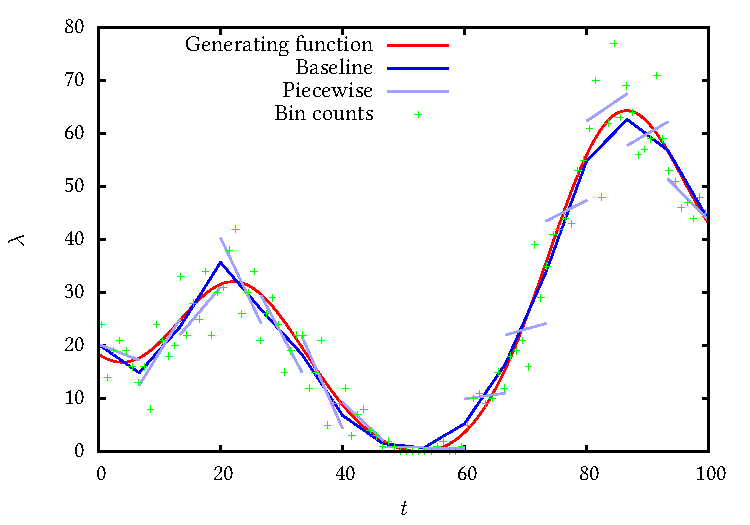
\includegraphics{pcbase}
    \caption{A comparison of the baseline and piecewise estimates on the same
    function.}
    \label{fig:basecomp}
    \end{figure}
\subsection{Kernel Density Estimation}
\label{sec-6-2}

   For comparison to the baseline estimator, a kernel density estimator was also
   implemented. A kernel density estimator works by estimating the function using
   multiple functions called kernels. We use a gaussian kernel 
   \begin{align}
   K(\mu,\sigma)=e^{-(t-\mu_i)^2/2\sigma_i^2}
   \end{align}
   to estimate the function. We centre a kernel at each photon arrival time $t_i$
   by setting $\mu_i=t_i$, which has been shown to be the best approach for this
   application \cite{cuevas2006accurate}. Once a kernel has been centred on each
   arrival time, the values of the kernels are summed at given points (depending on
   the sampling resolution) along the $x$-axis to form a function
   estimate. However, this is not the final step in the process. Depending on the
   standard deviation $\sigma$ of the kernels used, the estimated function
   $\hat{\lambda}(t)$ will be some multiple of the actual function
   $\lambda(t)$. Thus, we must normalise the value of the estimate. The
   normalisation constant is estimated by using the Poisson PDF. A range of
   possible normalisation constants is checked, and the one chosen is the value at
   which
   \begin{equation}
   \sum_{n=1}^N\frac{\lambda(t)^ke^{-\lambda(t)}}{k!}
   \end{equation}
   is minimised. We then apply this normalisation constant to $\hat{\lambda}(t)$
   when it is being used in calculations.
   \begin{figure}
   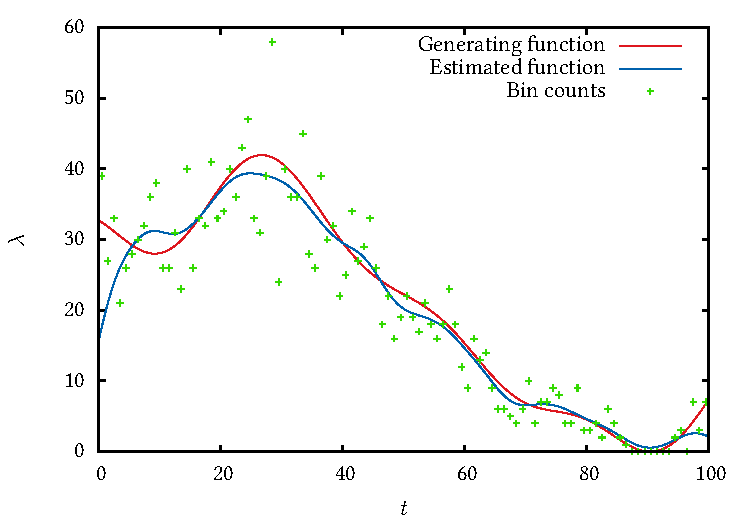
\includegraphics{gauss}
   \caption{Estimate of a function using Gaussian kernels. Note the drop-off at the
   start and end of the interval.}
   \label{fig:kde}
   \end{figure}
\subsection{Implementation}
\label{sec-6-3}

   Other than the libraries, the function estimators make up the largest portion
   of the system. As should be clear from what has been said above, the baseline
   estimator is built upon the IWLS estimator, and this is true in the code as
   well. The IWLS and OLS estimators form the base of the piecewise estimator,
   which is in turn used by the baseline estimator. The OLS estimator is
   implemented as a single iteration of the IWLS estimator; there is no separate
   code for OLS, apart from function which call the IWLS estimator with the
   correct parameters. The IWLS estimator first constructs arrays containing
   weights, bin counts and midpoints to be used in the estimation. At this
   stage, if there are no events in the interval that is being estimated, the
   estimator returns an empty estimate. Once the required arrays have been
   constructed, the estimator is simply a large loop which does all the required
   weight and constraint updates when required. The function returns a struct
   which contains the estimated values of $a$ and $b$, and the start and end of
   the interval that was being estimated. With OLS, the number of sub-intervals
   can be configured. For IWLS, in addition to the number of sub-intervals, the
   number of iterations can be set.

   The piecewise estimator uses a while loop to iterate through the given
   interval, which is split into sub-intervals by defining a maximum number of
   breakpoints. If the number of breakpoints is set to 4, then the maximum
   number of times the IWLS estimator will be called is 5---each breakpoint
   represents a point where the end of one interval meets the start of the
   next. During each iteration a function to extend the line estimated by
   IWLS. The process is hierarchical; if the initial extension fails, then a
   shorter interval is attempted. If no extension is possible after a given
   number of iterations, then extension fails. If the extension is successful,
   then the next interval estimate starts directly after the end of the extended
   estimate rather than its expected start point. In this way, it may be the
   case that there are fewer sub-intervals than expected based on the number of
   breakpoints. The line extension function requires the checking of event data
   in the interval it is attempting to extend into. Rather than reading the
   event file each time, a function was written which can, given a set of event
   data, return an array containing events within a desired interval. Each
   sub-interval estimate is stored in a struct which is simply an array of
   structs returned by the IWLS estimator.

   The baseline estimator takes the struct from the piecewise estimate and
   modifies the estimates inside it to ensure that the function produced by
   combining them is piecewise continuous. Four functions complete the
   process. First, the point at which the breakpoints occur is calculated. Then,
   the values of the two functions for the intervals before and after that point
   are calculated at the breakpoint. The midpoint of these two values is then
   calculated, and all functions for the sub-intervals are modified by drawing
   new lines between these points. The baseline and piecewise estimators have
   the same configuration parameters. The iterations and sub-intervals for the
   IWLS estimator to use, the maximum extension length, the maximum number of
   breakpoints, and the threshold value for the probability density function can
   be specified.

   The kernel density estimator uses is much simpler than the baseline
   estimator, using only two functions to perform all the operations
   required. The first stage is to generate an array of Gaussians using the
   event data---identical Gaussians centred on each event time, represented by
   their mean, standard deviation, and weight (set to 1). This array is then
   passed to a function which performs a discrete Gaussian transform on the
   array, by summing the Gaussians at points sampled at a given resolution. The
   function returns a two dimensional array containing the times of samples and
   their corresponding $\lambda$ values. A function which returns just the array
   of Gaussians is also used when all data on the Gaussians is required. The
   Gaussian estimator has only two parameters; the standard deviation of the
   Gaussian and the sampling resolution.
\subsubsection{Issues}
\label{sec-6-3-1}

    Initially, we thought that it may be possible to decide whether to
    extend the line or not based on the difference in slope between
    the estimate from the previous time interval and the estimate of
    the next. If the previous estimate was positive, and the next
    negative, and vice versa, clearly the line should not be
    continued. The intercept parameter was considered to be much less
    important. However, this assumption was highly flawed. Due to the
    nature of poisson processes, it is perfectly possible that
    although the function has changed significantly after the end of
    the previous interval, the estimate for the interval that we are
    trying to extend the line into could return very similar values to
    that of the previous interval. Because of this, we extend the line
    when we should not be doing so. There are several potential
    solutions to this problem. First, rather than forming a new
    estimate, we extend the line and then check how much the error has
    increased. If it goes over a certain threshold, then we reject the
    extension attempt and try again, this time with a shorter
    extension. Another potential way of improving the piecewise
    estimation in general would be to require the estimate for the
    next time period to start from the end point of the last time
    period. This would prevent the intercept parameter from changing,
    and would force the estimator to find the best estimate given a
    specific starting point, rather than giving it free reign to find
    the estimate which actually minimises the error.
\section{Time Delay Estimation}
\label{sec-7}

  Once we are able to estimate the characteristic function of photon streams, we
  can use these estimates to compute an estimate of the time delay between two
  streams. If the two streams come from the same source, then they should have the
  same characteristic function with some delay $\Delta$. Our estimates of the
  characteristic function will differ for both streams due to the fact that the
  number of photon arrivals in each bin will be different for each stream, but
  each should look relatively similar. In this section we present two methods for
  estimating the time delay between a pair of streams based on their function estimates.
\subsection{Area Method}
\label{sec-7-1}

   The first of the two methods uses a very simple metric to estimate the time
   delay. By taking the two function estimates, we can attempt to match up the two
   functions so that they ``fit together'' best. This goodness of fit can be
   determined by the area between the two functions. The point at which the area
   between the two is lowest is the natural point at which the two functions should
   match. Using the first estimate as a base, with its time delay set to zero, we
   guess at values of $\Delta$ between $-\Delta_{\text{max}}$ and
   $+\Delta_{\text{max}}$, and shift the second estimate by that value. Then, we
   calculate the area between the function estimates area using
   \begin{align}
   \begin{split}
   d(\hat{\lambda}_1,\hat{\lambda}_2)&=\int(\hat{\lambda}_1(t)-\hat{\lambda}_2(t))^2\,dt\\
   &\approx\frac{1}{N}\sum_{i=1}^N(\hat{\lambda}_1(t)-\hat{\lambda}_2(t))^2
   \end{split}
   \end{align}
   We use the value of $\Delta$ at which $d(\hat{\lambda}_1,\hat{\lambda}_2)$ is
   minimised as the time delay estimate. Rather than using an integral to get the
   exact area between the functions, we use a less computationally expensive
   discrete approximation. Figure \ref{fig:areamethod} gives a basic idea of the
   logic behind the method.
   \begin{figure}
   \subfloat[High area ($\Delta=$ 0)]{
   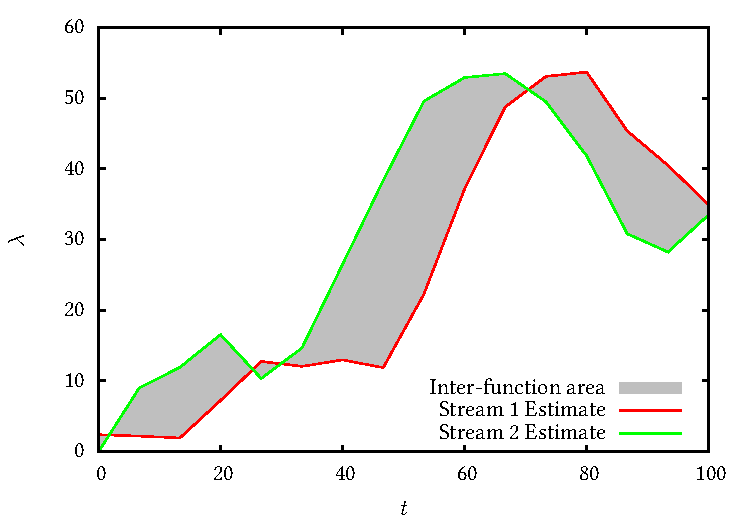
\includegraphics{normarea}
   }\\
   \subfloat[Low area ($\Delta=$ 13.3)]{
   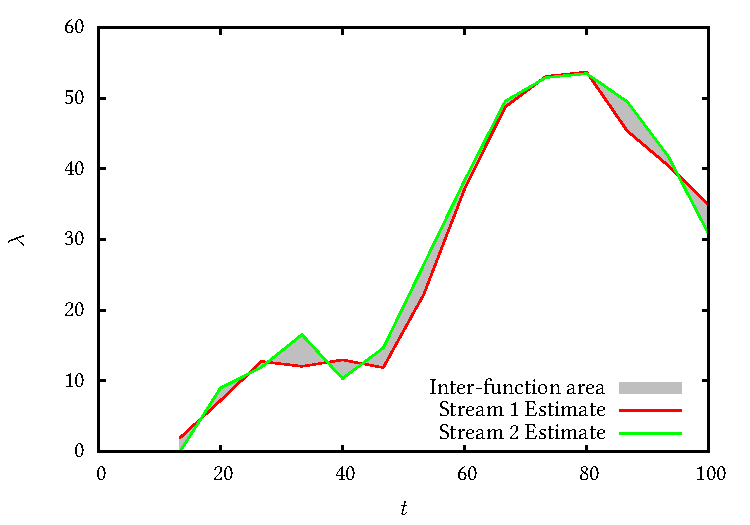
\includegraphics{shiftarea}
   }
   \caption{Comparison of area between functions for two different values of
   $\Delta$. Note that calculation of area is only possible in overlapping
   regions---the first 13.3 time units must be ignored in (b). A smaller area
   clearly indicates a better match.}
   \label{fig:areamethod}
   \end{figure}
\subsection{Probability Density Function Method}
\label{sec-7-2}

   The second method of estimation is using probability density functions. As
   before, we guess a value of $\Delta$ between $-\Delta_{\text{max}}$ and
   $+\Delta_{\text{max}}$ and shift the second stream by that amount. However, we
   know that there must be a single characteristic function, and we want to see how
   well our estimate of that matches the bin counts in each stream. From the two
   stream estimates we have, $\hat{\lambda}_1$ and $\hat{\lambda}_2$ (which is
   shifted by $\Delta$), we make an ``average'' function $\bar{\lambda}$ by combining the
   two.
   \begin{equation}
   \bar{\lambda}(t)=\frac{\hat{\lambda}_1(t)+\hat{\lambda}_2(t+\Delta)}{2}
   \end{equation}
   The point on $\bar{\lambda}$ at time $t$ is the midpoint between the values of
   the two estimates at that time. Once we have $\bar{\lambda}$, we can assign some
   score to the current estimate of the value of $\Delta$.
   \begin{align}
   \begin{split}
   \log P(S_A,S_B\mid\bar{\lambda}(t))=\sum_{t=\Delta_{\text{max}}}^{T-\Delta_{\text{max}}}&\log P(S_A(t)\mid \bar{\lambda}(t))\\
   &+ \log P(S_B(t+\Delta)\mid \bar{\lambda}(t))
   \end{split}
   \end{align}
   Here, we calculate the probability that the function $\bar{\lambda}$ is the
   characteristic function of the two streams $S_A$ and $S_B$. The streams are
   split into bins, and the probability of the number of events in each bin given
   the value of $\lambda$ calculated for that bin is computed. 

   \textcolor{red}{Perhaps this should go in the previous section} It is important
   to note that the value of $\Delta_{\text{max}}$ defines the interval in which
   the probabilities are summed. The need for calculation only in some specific
   interval should be clear---if one function is shifted, and both functions have
   the same time interval, then there will be an interval of $\Delta$ on either end
   of the range in which only one of the functions has a value. As such, the
   functions are combined only in the interval in which both functions have
   values. In addition to this, since the value of $\Delta$ changes, the intervals
   in which there is an overlap between the two functions changes. Setting
   $\Delta=0$ minimises the value, and $\Delta=\pm\Delta_{\text{max}}$ maximises
   it. To be able to compare the scores of different values of $\Delta$, we must
   perform calculations on the interval in which the two functions have values for
   all possible values of $\Delta$. If the calculations were to be performed on
   different intervals or interval lengths each time, it would be necessary to
   scale the scores for the longer intervals to the shorter intervals, and this
   scaling would likely not result in an accurate representation of the actual
   score. Imposing this constraint on the intervals we can work with has an
   additional effect; the value of $\Delta_{\text{max}}$ can never exceed the
   interval length $T$ in which we are performing the estimate. We are left with
   the constraints $T_{\text{est}}=[t_0+\Delta_{\text{max}},
   T-\Delta_{\text{max}}],\,\Delta_{\text{max}}<T$ on the interval and the maximum
   value of $\Delta$.

   The calculation of $\lambda$ is slightly more complicated than just taking the
   value of lambda at the midpoint. Since we are considering a number of events
   occurring in a given time span, we must consider the value of lambda in that
   entire time interval. In order to do this, we integrate the value of lambda over
   the interval
   \begin{equation}
   \lambda_{a,b}=\int_a^b\lambda(t)\,dt
   \end{equation}
   However, as with the calculation of the area between curves, we do not need an
   exact value, only a good approximation, and so we use a discrete version of this
   equation where the value of $t$ is incremented by some finite step for each successive
   value. The smaller the value of the step the more accurate the approximation of
   $\lambda_{a,b}$ becomes. As with the previous estimator, the estimate is made in
   two stages, first with a coarse pass over the values of delta to compute an
   initial estimate, and then a finer second pass around the first estimated value
   in order to refine the estimate.
\subsection{Implementation}
\label{sec-7-3}

   Both the area and PDF methods perform the same hierarchical estimate of the
   time delay. As always, the first stage of the process is to extract required
   parameters. Once the initial estimate is received, the process is simply
   repeated with a slight change in the parameters to the function to make the
   second, finer pass over the data. Since both the methods may receive data
   from either of the two function estimation methods, they use a void pointer
   to receive the estimate data, and take a switch that is used to select the
   correct function to process the data. The estimate data is cast to the
   correct type before it is processed. Each of the functions returns a single
   double precision value of the estimate it makes.

   To produce its estimate, the PDF estimator must combine the two function
   estimates into a single function. The different function estimates are stored
   in different data types, so a separate function is used for each
   type. The function can in theory combine any number of streams, but has only
   been tested to a maximum of 4. One of the parameters it takes is an array of
   time delays, which is used to shift the function in time before combination
   takes place. 

   The time delay estimation must somehow be combined with the function
   estimation. This is done by the \texttt{multi\_estimate} function. Again, this
   is a two stage function, the first stage of which extracts the relevant
   parameters. Depending on the type of estimator, different parameters are
   retrieved. The function can do estimates of several functions with only a
   single call by using the standardised output filenames. The second stage of
   the function first estimates the characteristic function of each stream
   (tested up to 4 streams). If the kernel density method is being used, a
   normalisation constant is calculated. Finally, the time delay estimate is
   performed using the estimates and the normalisation constant (if
   required). Using the best scoring estimates between each stream, the
   functions for all streams are combined to make a single final estimate of the
   function, which is both output to file and returned to the caller.

   The parameter file contains several parameters for configuring the time delay
   estimators. The estimation can be turned on or off, and the method can be
   chosen. It is also possible to specify whether to use the hierarchical
   estimation method. A step for the first and second pass can be specified, as
   well as the range in which to check. The sample resolution must be specified
   for both the area and PDF estimators, and the PDF estimator also requires the
   number of bins into which it is to split the interval.
\section{Experimentation}
\label{sec-8}

  \begin{figure}[h!tb]
  \subfloat[$\alpha=0.005$]{
  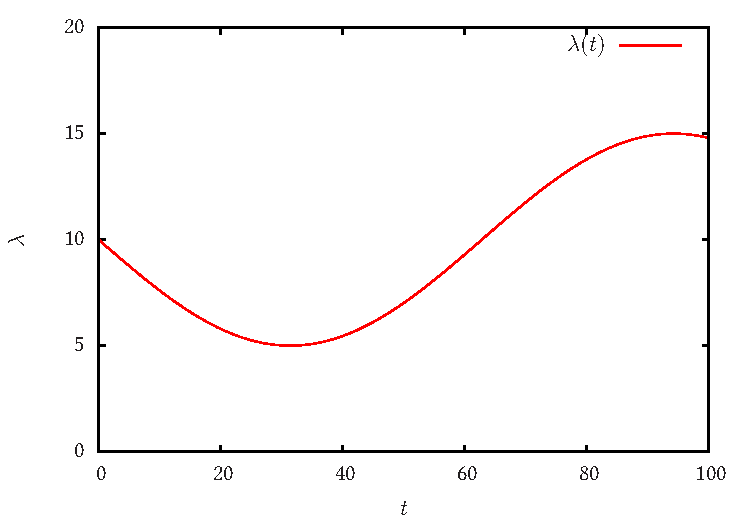
\includegraphics[width=0.5\textwidth]{prelim_sine_005}
  }
  \subfloat[$\alpha=0.01$]{
  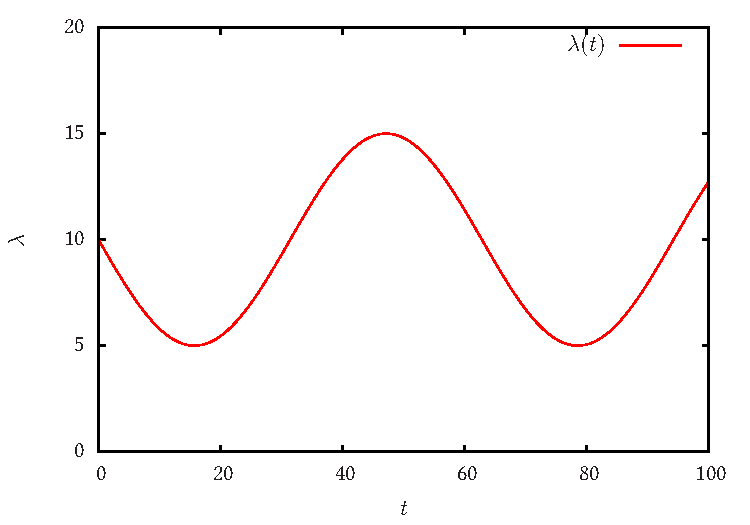
\includegraphics[width=0.5\textwidth]{prelim_sine_01}
  }\\
  \subfloat[$\alpha=0.015$]{
  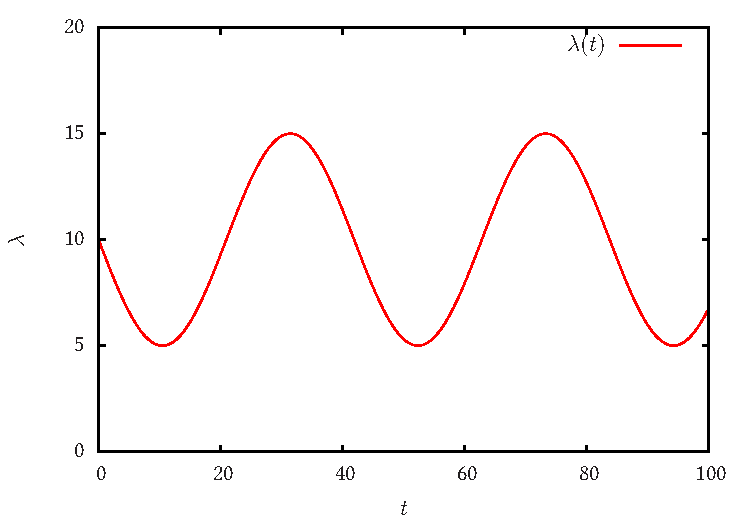
\includegraphics[width=0.5\textwidth]{prelim_sine_015}
  }
  \subfloat[$\alpha=0.03$]{
  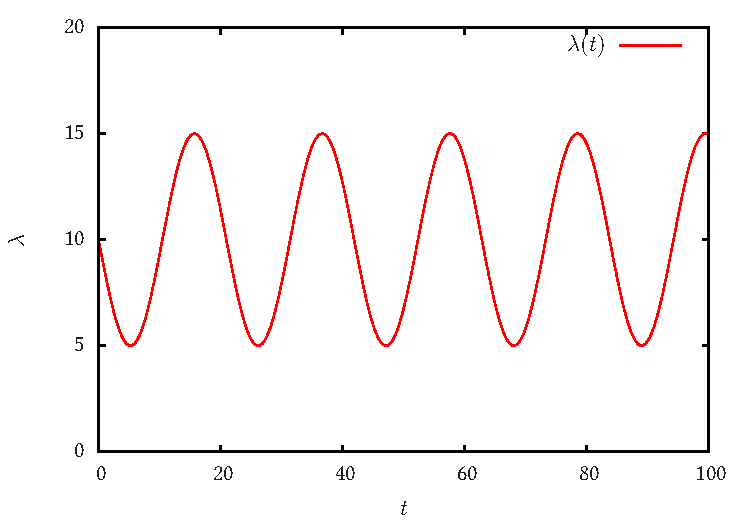
\includegraphics[width=0.5\textwidth]{prelim_sine_03}
  }\\
  \begin{center}
  \subfloat[$\alpha=0.06$]{
  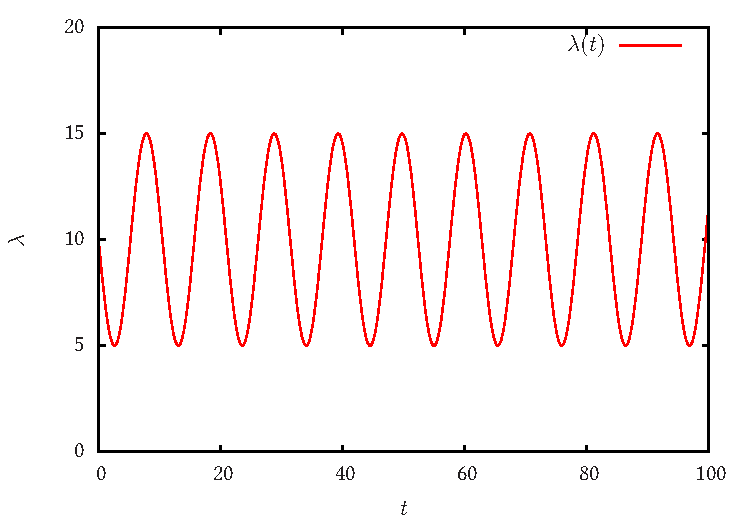
\includegraphics[width=0.5\textwidth]{prelim_sine_06}
  }
  \end{center}
  \caption{Functions used for preliminary experiments on sine functions, showing
  the different $\alpha$ values used. The generating function is $y=a-b\sin(\alpha t)$.}
  \label{fig:avals}
  \end{figure}
  The experiments done have two stages. First, the optimum parameter set for each
  function that is being experimented on is found using model selection. Model
  selection involves withholding some of the data from the estimator so that we
  can see how well a parameter set generalises if not all the data is
  available. Withholding data is done by removing the event data from intervals
  uniformly distributed across the interval that is being estimated. Each function
  is estimated, and the value of the function in the regions where data was
  removed is compared to the value that would be expected had all the data been
  present. This is done using log probabilities, taking the Poisson PDF at each
  point. The sum of these log probabilities gives the parameter set its score for
  that function. The optimum parameter set for that function is the set which
  maximises the sum.

  The Gaussian estimator was set to sample the kernels at a resolution of 0.3 time
  steps, and the standard deviation of the kernels was varied. The baseline
  estimator was set to use 3 iterations of the IWLS estimator, and four other
  parameters were experimented on.
  \begin{description}
  \item[IWLS sub-intervals] 2, 4, 6, 8, 10
  \item[PDF threshold] 0.01 to 0.15 with a step of 0.01
  \item[Maximum extension] 5, 7, 9, 11, 13, 15, 17, 19, 20
  \item[Maximum breakpoints] As above
  \item[Gaussian standard deviation] 0.5 to 20 with a step of 0.5
  \end{description}
  The parameters were co-varied, meaning that each value for one
  of the parameter settings was tested with all possible values of the other
  parameters, for a total of 6115 possible combinations.

  Once the optimum parameter set has been found, the time delay
  for the pair of streams is estimated, using all the data that is available. From
  this we receive estimates of the time delay on which it is possible to perform
  statistical analysis. The mean, standard deviation and error for each estimate
  on each function is calculated, and from this we can examine the effectiveness
  of the estimates. The aim of the experimentation is to compare the effectiveness
  of the time delay estimation with four combinations of estimators: gaussian
  area, gaussian pdf, baseline area and baseline pdf. For the full set of
  experimental data, see Appendix \ref{sec-11}.

  We assume that the distribution of the samples is Gaussian, but this may not be
  the case. However, full non-parametric testing is out of the scope of this project.
\subsection{Sine Functions}
\label{sec-8-1}

   The first experiment performed was on sinusoidal functions of the form
   $y=a-b\sin(\alpha t)$. An increase in the value of $\alpha$ increases the
   oscillation frequency, and a decrease reduces it. The value of $a$ indicates how
   much the wave is shifted along the $y$-axis, and $b$ determines the
   amplitude of the wave. The values of $a$ and $b$ were set to 10 and 5 respectively.
\subsubsection{Preliminary Experiments}
\label{sec-8-1-1}

    In the first set of experiments, we investigate the performance of the
    estimators on five values of $\alpha$: 0.05, 0.1, 0.15, 0.3 and 0.6. Figure
    \ref{fig:avals} gives an indication of what the functions look like. For
    each value of $\alpha$, 25 pairs of streams were independently generated, each
    with an interval of 100 time units and a time delay of 10 time steps between the
    two streams. 

    Estimates appear to be reasonably accurate until $\alpha$ exceeds 0.1, after
    which errors become much greater, and standard deviation increases. The area
    time delay estimator is significantly better than the PDF for both of the
    function estimators, with $p$-values of 0.00017 and 0.0000074 for the baseline
    and Gaussian method respectively at $\alpha=$ 0.05. The difference between the
    two function estimation methods was not significant, with $p$-values in excess
    of 0.4 for comparisons between the baseline and Gaussian estimators for the same
    time delay estimators at $\alpha=$ 0.05. Results from $\alpha>$ 0.005 show no
    statistical significance in the difference between the various estimators, so
    although the $p$-values at $\alpha$ =0.05 are significant, they are not
    sufficient to say that the area estimator is always better. Figure
    \ref{fig:prelimerror} shows the error of the various estimator combination at
    each value of alpha.
    \begin{figure}
    \subfloat[Baseline area]{
    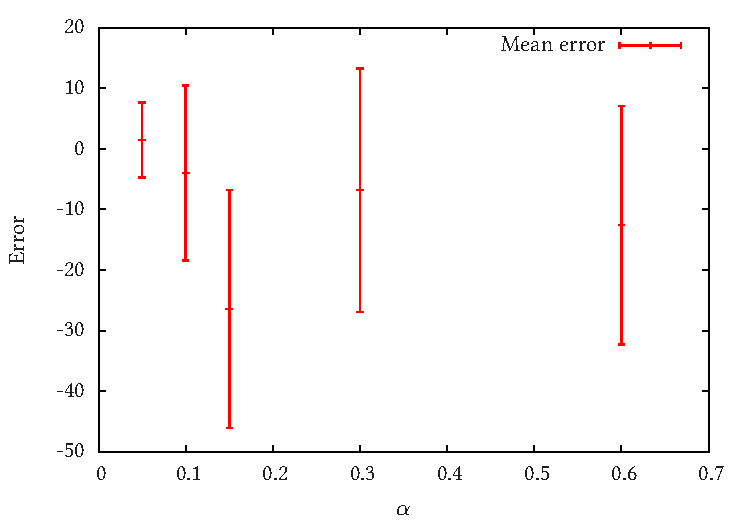
\includegraphics[width=0.5\textwidth]{base_area_prelim}
    }
    \subfloat[Baseline PDF]{
    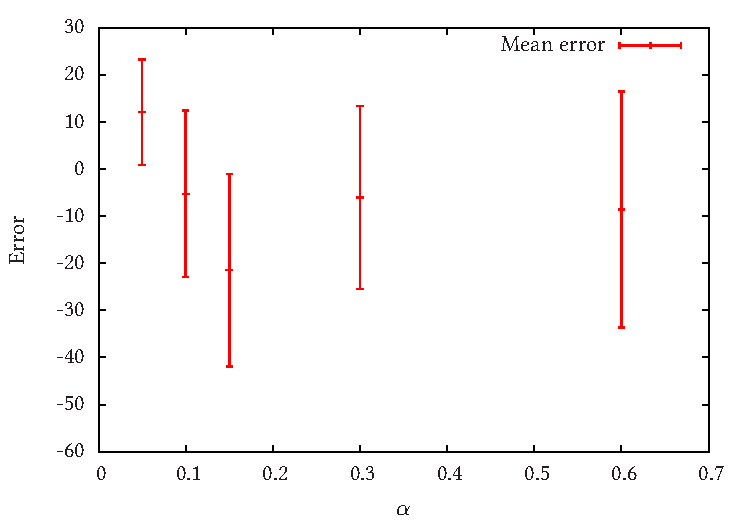
\includegraphics[width=0.5\textwidth]{base_pmf_prelim}
    }\\
    \subfloat[Gaussian area]{
    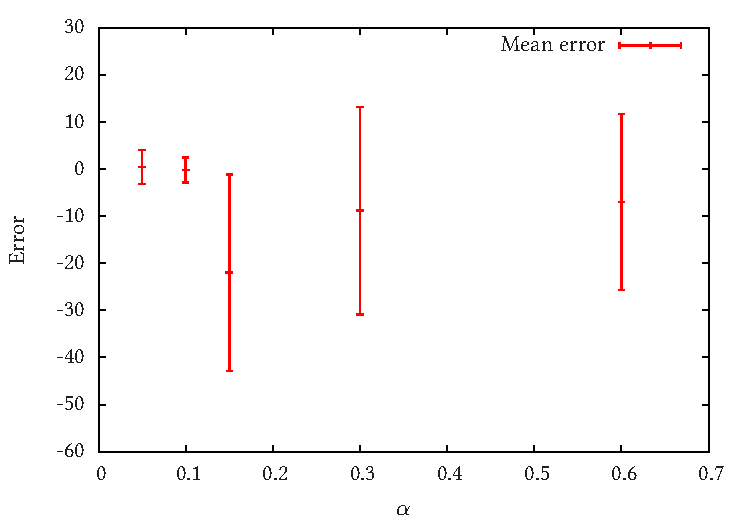
\includegraphics[width=0.5\textwidth]{gauss_area_prelim}
    }
    \subfloat[Gaussian PDF]{
    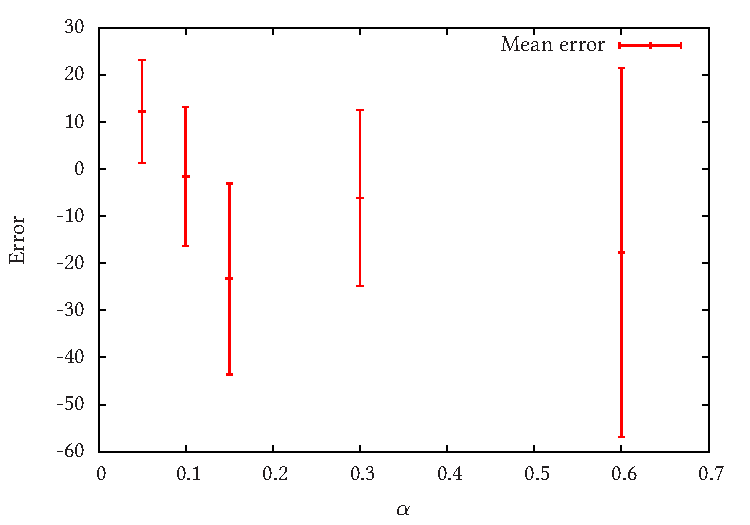
\includegraphics[width=0.5\textwidth]{gauss_pmf_prelim}
    }
    \caption{Error on the preliminary experiments. Error bars show standard
    deviation of error. Performance appears to deteriorate when $\alpha>0.1$.}
    \label{fig:prelimerror}
    \end{figure}
\begin{table}[htb]

\begin{center}
\begin{tabular}{l|ll}
       &  Gaussian           &  Baseline           \\
\hline
 Area  &  10.39 $\pm$ 3.60   &  11.43 $\pm$ 6.18   \\
 PDF   &  22.20 $\pm$ 10.94  &  22.06 $\pm$ 11.20  \\
\end{tabular}
\end{center}
\caption{Experimental results for $\alpha=$ 0.05. Actual time delay is 10. ($\mu\pm\sigma$)} \label{fig:pretab}\end{table}
\subsubsection{Refined Experiments}
\label{sec-8-1-2}

    Although the previous set of experiments provide some indication as to the
    performance of the estimators, we investigated their effectiveness on a smaller
    range of $\alpha$ values. In this set of experiments, we used the same
    parameters, but generated a new set of functions for value of $\alpha$ from
    0.01 to 0.15, with a step of 0.01 between each successive set of stream
    pairs. For each value of $\alpha$, 10 pairs of streams were generated. The time
    delay was set to 15 time steps, and the experiments were run with the same set
    of experimental parameters as the previous experiments.

    The result of this second set of experiments uncovered an interesting pattern in
    the performance of the estimators. Figure \ref{fig:fineerror} shows the error
    for each combination of estimators for different values of $\alpha$. It is clear
    to see from the graphs that there is a window of optimum performance where
    $\alpha$ is between 0.04 and 0.1. As with the previous set of experiments, the
    area estimator again outperforms the PDF estimator, which is visible in the
    graphs. Within this window, the area method is significantly better than the PDF
    estimator in some cases, but this significance varies greatly as $\alpha$
    varies, and we therefore cannot conclude that there is a definite increase in
    accuracy using the area method. As before, the Gaussian and baseline methods do
    not differ significantly in performance, but on average the Gaussian method
    performs slightly better, having smaller standard deviations than the area
    method.
    \begin{figure}
    \subfloat[Baseline area]{
    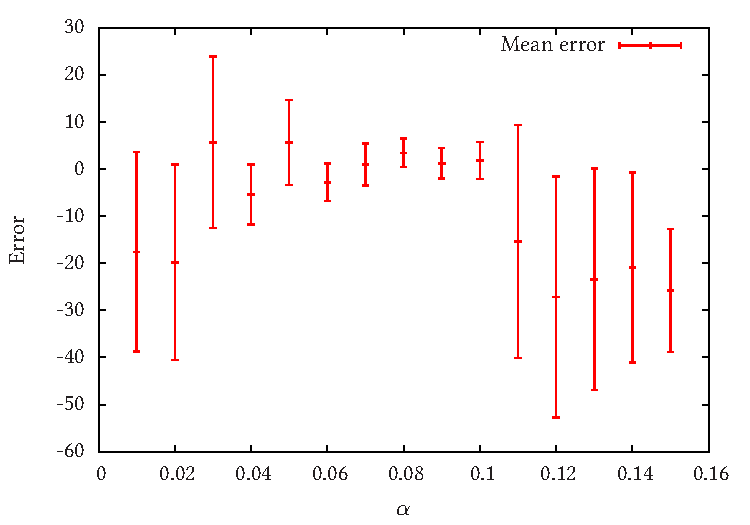
\includegraphics[width=0.5\textwidth]{baseline_area_fine}
    }
    \subfloat[Baseline PDF]{
    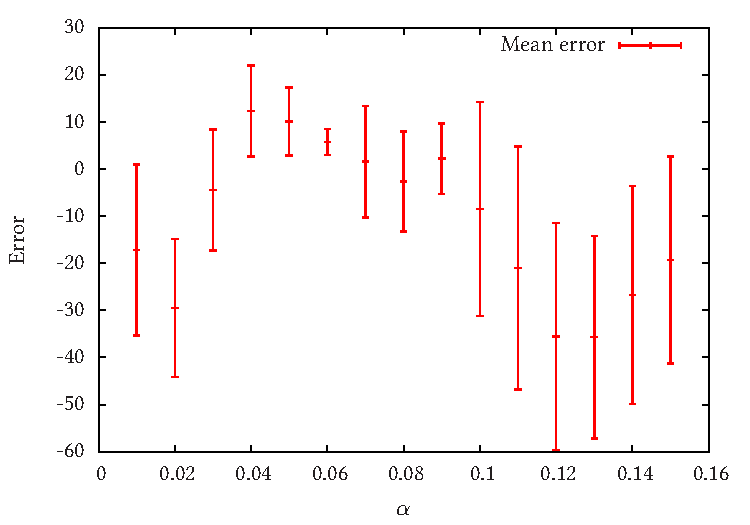
\includegraphics[width=0.5\textwidth]{baseline_pmf_fine}
    }\\
    \subfloat[Gaussian area]{
    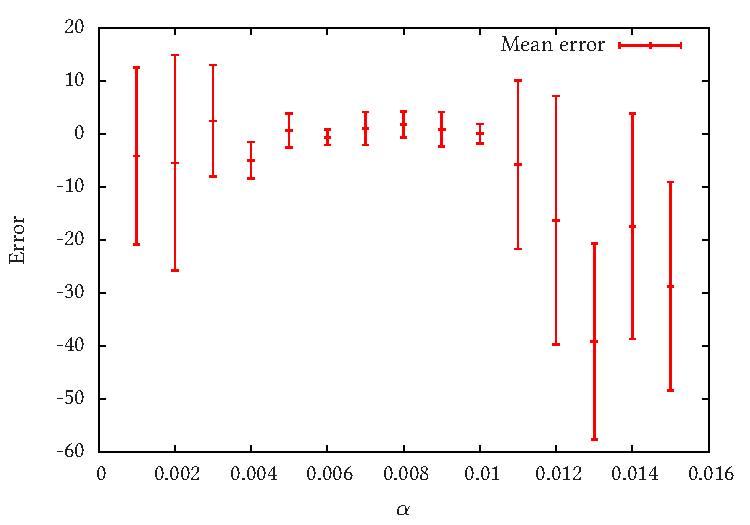
\includegraphics[width=0.5\textwidth]{gaussian_area_fine}
    }
    \subfloat[Gaussian PDF]{
    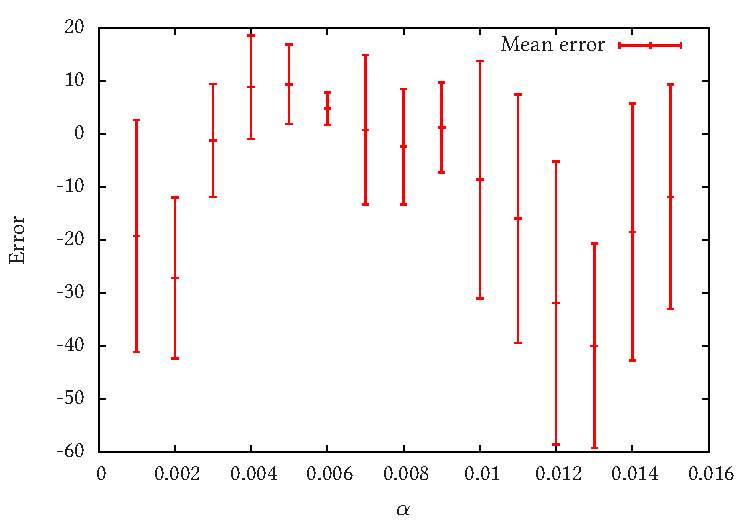
\includegraphics[width=0.5\textwidth]{gaussian_pmf_fine}
    }
    \caption{Error on the second set of experiments. Error bars show
    standard deviation of error. Peak performance is in the window 0.04
    $\leq\alpha\leq$ 0.1}
    \label{fig:fineerror}
    \end{figure}
\subsection{Random Functions}
\label{sec-8-2}

   The experiments on sine functions have not yielded any definitive result as to
   which methods are more effective, and so we also performed a series of
   experiments using random functions rather than sine curves. Evaluating the
   performance of the estimator on these functions is important, since functions
   from real lensed objects will be very unlikely to follow a perfect sine curve,
   instead fluctuating somewhat randomly. In order to test a variety of different
   functions, vary the $\alpha$ parameter in the equation $\sigma=\alpha\cdot\Delta
   t$, where $\sigma$ is the standard deviation of the Gaussians used to generate
   the random function. The weight of each Gaussian was set to 3, to give a larger
   range of shapes that the function could take on.
   \begin{center}
   \begin{figure}
   \subfloat[$\alpha=0.4$]{
   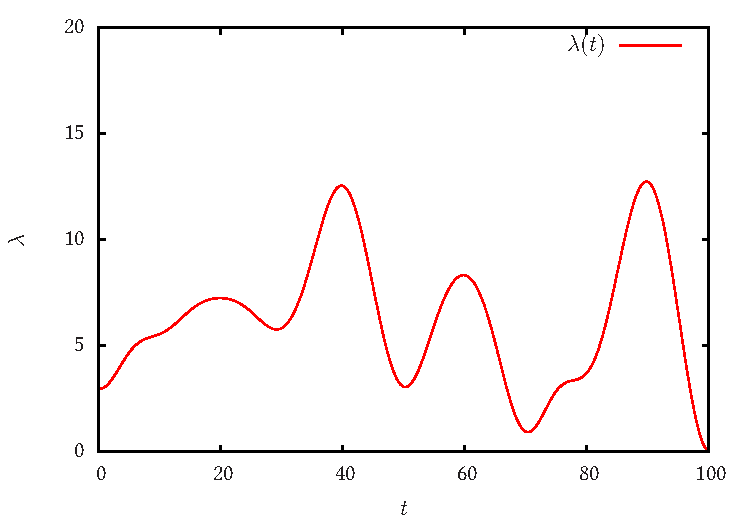
\includegraphics[width=0.5\textwidth]{randfunc_04}
   }
   \subfloat[$\alpha=0.8$]{
   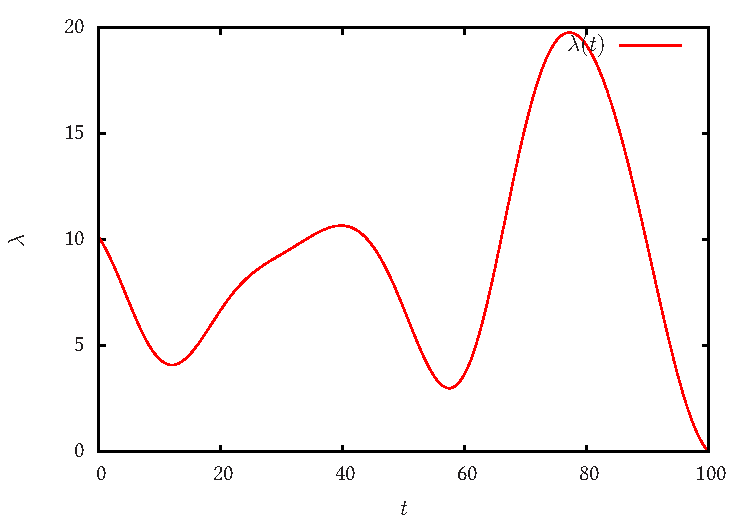
\includegraphics[width=0.5\textwidth]{randfunc_08}
   }\\
   \subfloat[$\alpha=1$]{
   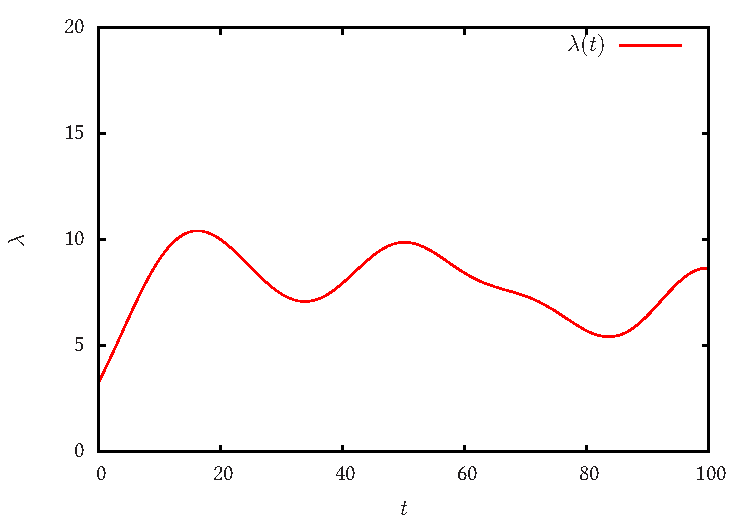
\includegraphics[width=0.5\textwidth]{randfunc_1}
   }
   \subfloat[$\alpha=2$]{
   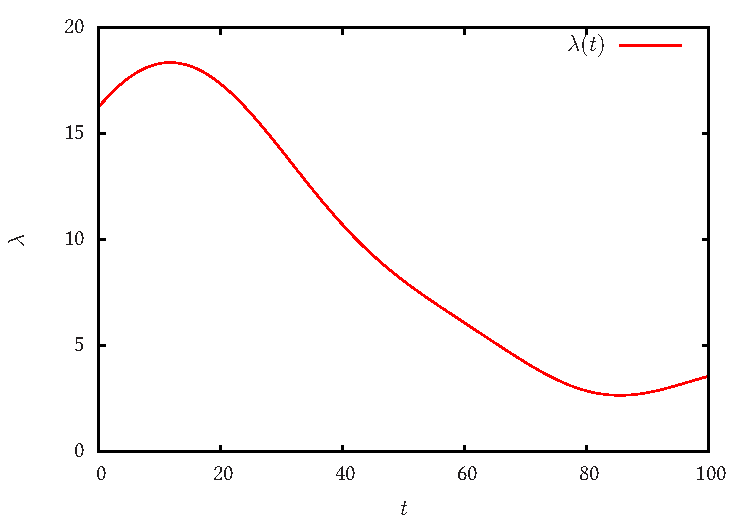
\includegraphics[width=0.5\textwidth]{randfunc_2}
   }\\
   \begin{center}
   \subfloat[$\alpha=3$]{
   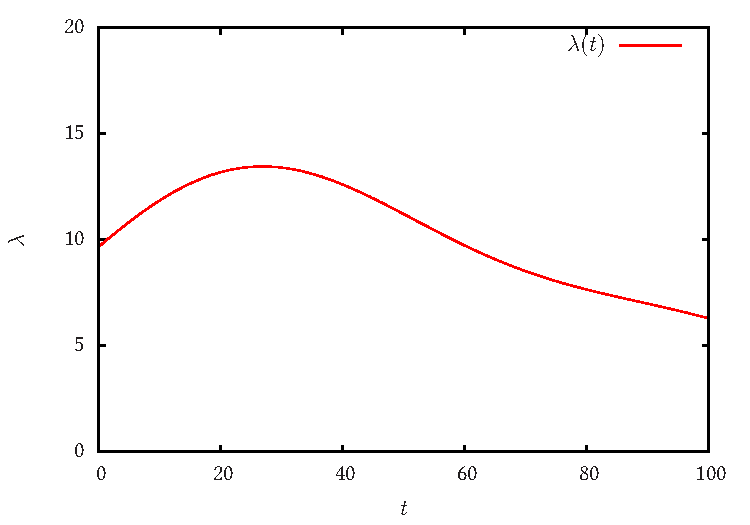
\includegraphics[width=0.5\textwidth]{randfunc_3}
   }
   \end{center}
   \caption{Examples of random functions generated by different
   values of $\alpha$. Oscillation of the functions decreases as $\alpha$ increases.}
   \label{fig:randex}
   \end{figure}
   \end{center}
\subsubsection{Preliminary Experiments}
\label{sec-8-2-1}

    For the preliminary experiment, we chose to use five different values of
    $\alpha$, 0.4, 0.8, 1, 2 and 3. While increasing the $\alpha$ parameter in the
    previous set of experiments would make the functions more difficult to estimate,
    in this case the opposite is true; larger values are easier to estimate, whereas
    smaller values are more difficult. This is due to the relationship of $\alpha$
    and the standard deviation of the Gaussians used to generate the functions. For
    the preliminary experiments we set the value of $\Delta t$ to be 10, resulting
    in 11 Gaussians being spread uniformly across the 100 time unit interval. Given
    that $\alpha$ ranges from 0.4 to 3, the value of $\sigma$ will be between 4 and
    30 time units. Lower values of $\sigma$ result in each Gaussian being spread
    over a smaller interval, which in turn means that when the Gaussians are summed
    to construct the function it will have more variation than with large values. We
    generated 5 different functions for each value of $\alpha$, and from each of
    these generated 5 pairs of photon streams. In these initial experiments, we wish
    to discover where the point of deterioration is, so that we can look at the
    region close to this in more detail in a subsequent set of experiments.

    The results from the experiment were very enlightening. Figure
    \ref{fig:randerror} shows the error of the estimators over all $\alpha$
    values. The estimators performed with much smaller error values on average,
    leading us to believe that the large errors in the previous experiments were due
    to the shape of the functions. The methods that we use seem to be ineffective on
    functions which have a symmetrical shape, which sine functions are. The
    estimators appear to be much more stable, with the mean error deviating
    relatively little from zero, in comparison to the wild variation in the sine
    function experiments. While the performance of the estimators was better, the
    difference between method combinations is still not significant. The large error
    at $\alpha$ is 1 is due to very large errors occurring in estimates of two
    functions in that data set. This indicates that while on average the estimators
    perform well, on functions with certain characteristics there are large
    differences in the performance. Both time delay estimation methods perform worse
    when $\alpha$ is 0.4, but the estimate from the area method is clearly less
    affected.
    \begin{figure}
    \subfloat[Baseline area]{
    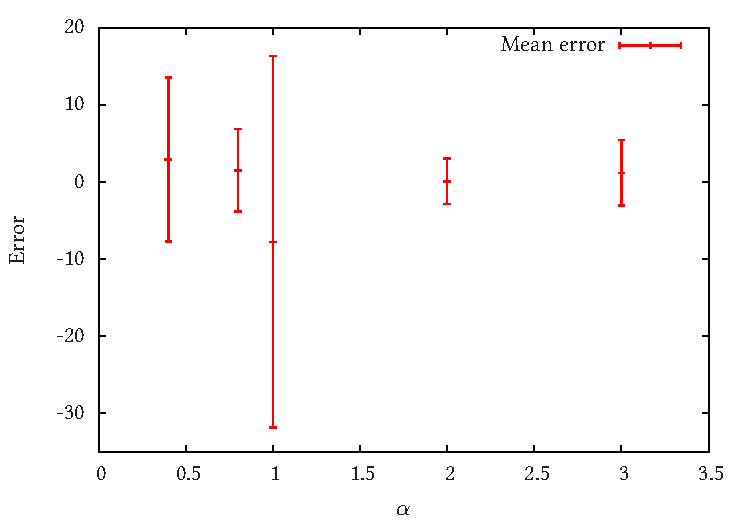
\includegraphics[width=0.5\textwidth]{baseline_area_random}
    }
    \subfloat[Baseline PDF]{
    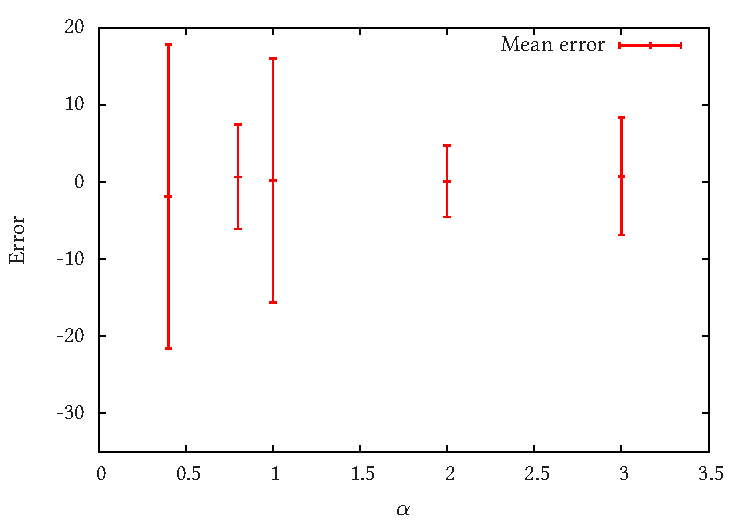
\includegraphics[width=0.5\textwidth]{baseline_pmf_random}
    }\\
    \subfloat[Gaussian area]{
    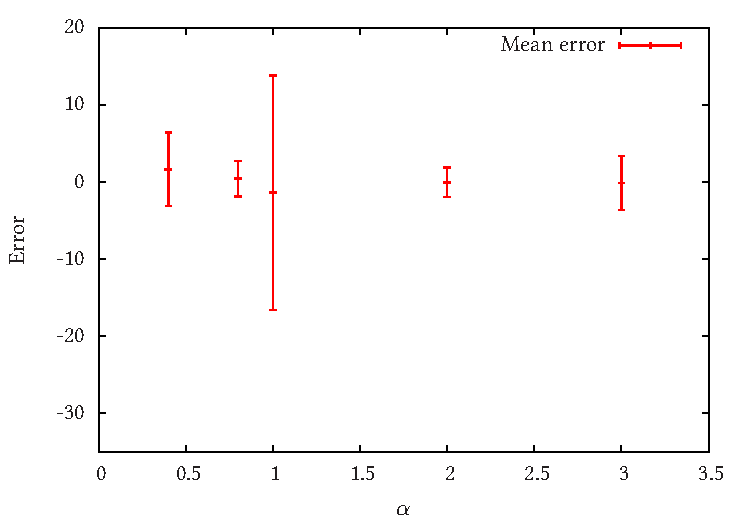
\includegraphics[width=0.5\textwidth]{gaussian_area_random}
    }
    \subfloat[Gaussian PDF]{
    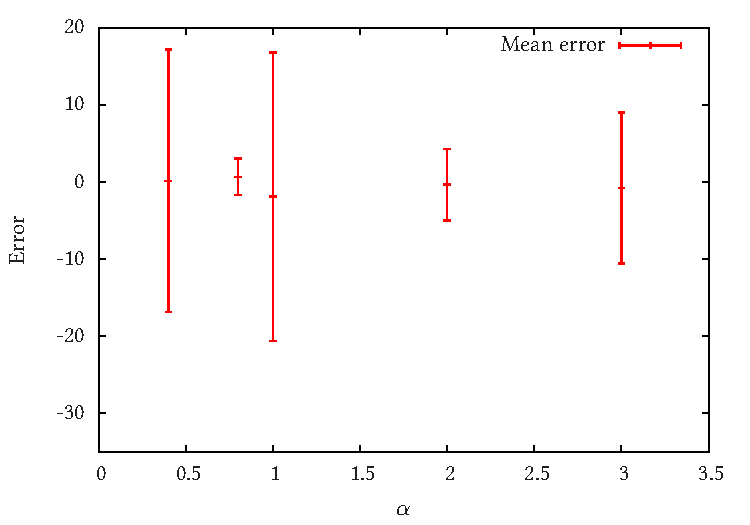
\includegraphics[width=0.5\textwidth]{gaussian_pmf_random}
    }
    \caption{Mean error for each value of $\alpha$ for the preliminary random
    function experiments for each method combination.}
    \label{fig:randerror}
    \end{figure}
\subsubsection{Refined Experiments}
\label{sec-8-2-2}

    In order to investigate the estimator performance further, we performed an
    additional experiment on a finer set of data, varying $\alpha$ from 0.1 to 1.5,
    with steps of 0.1. Going down to such a low value of $\alpha$ results in
    functions which have very large variations, with impulse-like peaks and troughs,
    an example of which can be seen in Figure \ref{fig:smallalpha}. The parameter
    ranges used were the same as in the previous experiment on random functions.

    This experiment confirms our observation from the previous experiment that the
    Gaussian area method combination is the one which should be used to get the best
    estimates with the smallest errors, which is clear to see in Figure
    \ref{fig:moreranderror}. Again, there was no pattern in the $p$-values that
    could be said to indicate that one method is significantly better than another,
    so we can not conclude with certainty that the Gaussian area method is indeed
    better than the others. However, this and previous experiments have shown that
    the size of the error from estimates with that combination is in the vast
    majority of cases smaller than that of other combinations. Errors appearing in
    combinations using the PDF method increase as values of $\alpha$ drop below 0.4,
    indicating that the method is more error-prone when functions have large
    variations. The PDF method in general has larger standard deviations on the
    error than the area method.
    \begin{figure}
    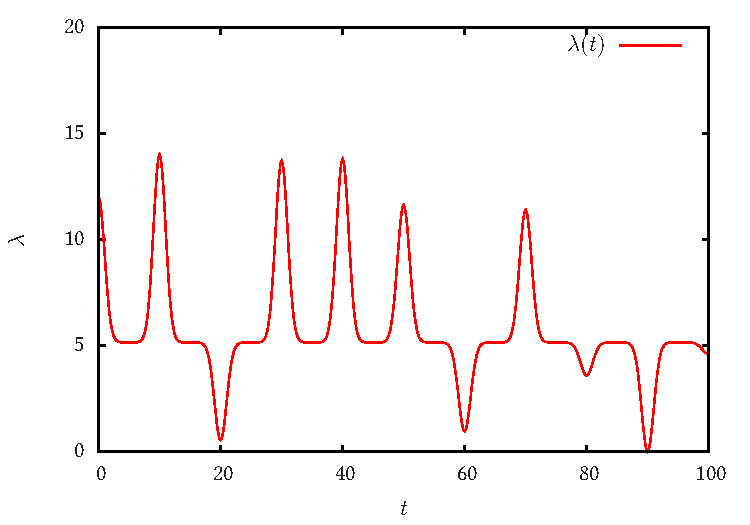
\includegraphics{smallalpha}
    \caption{Example of a function generated with $\alpha$ set to 0.1. The straight
    line at $\lambda=$ 5 is a result of the function being shifted to make all values
    $\geq 0$.}
    \label{fig:smallalpha}
    \end{figure}

    \begin{figure}
    \subfloat[Baseline area]{
    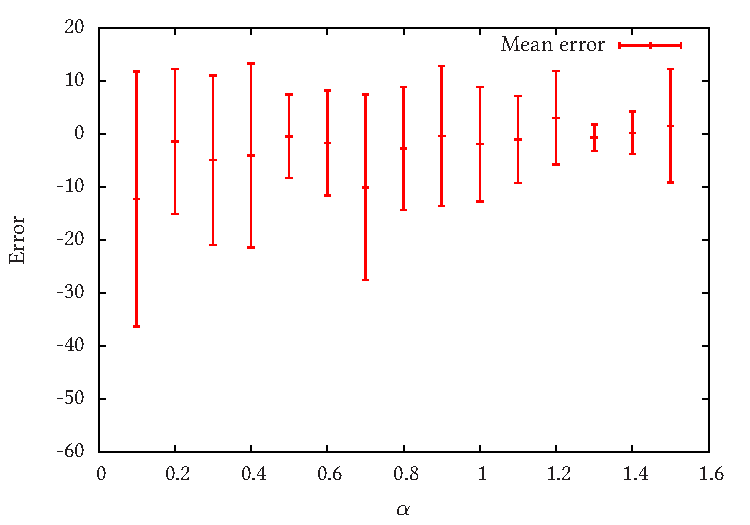
\includegraphics[width=0.5\textwidth]{baseline_area_morerand}
    }
    \subfloat[Baseline PDF]{
    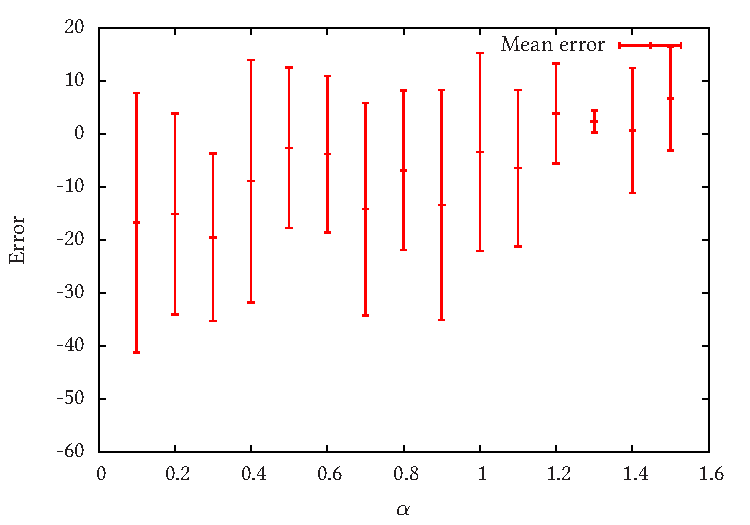
\includegraphics[width=0.5\textwidth]{baseline_pmf_morerand}
    }\\
    \subfloat[Gaussian area]{
    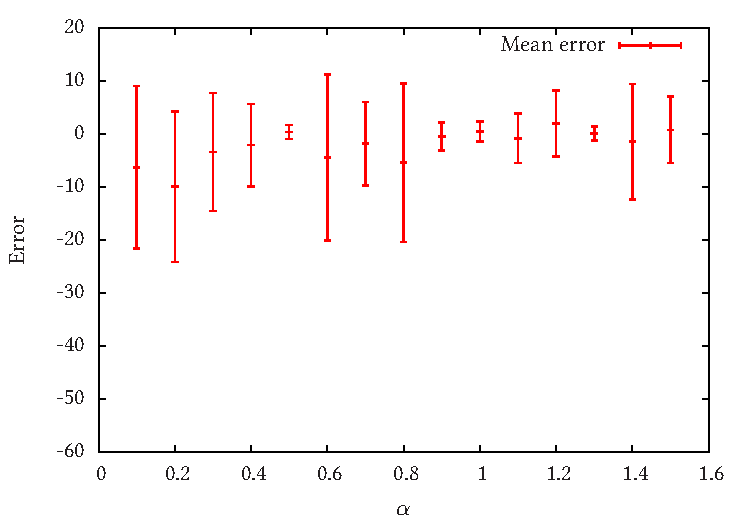
\includegraphics[width=0.5\textwidth]{gaussian_area_morerand}
    }
    \subfloat[Gaussian PDF]{
    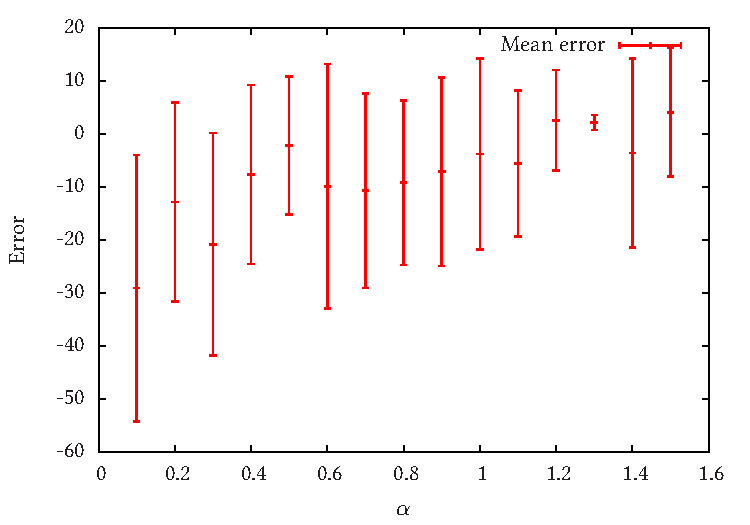
\includegraphics[width=0.5\textwidth]{gaussian_pmf_morerand}
    }
    \caption{Mean error for each value of $\alpha$ for the second set of random
    function experiments for each method combination.}
    \label{fig:moreranderror}
    \end{figure}
\section{Conclusion}
\label{sec-9}

  In this report, we have presented our system for estimating the time delay in
  gravitationally lensed photon stream pairs. We showed two methods for estimating
  the characteristic function of the stream; the baseline method, which is build
  upon the iterative weighted least squares method, and the Gaussian kernel
  density estimation method. In addition, we presented two methods for time delay
  estimation, one using inter-function area, and another using probability density
  functions. 

  We performed two experiments on sine functions with different
  oscillation frequencies. The first showed that there appeared to be a point of
  deterioration at which the estimators' performance experienced a large
  decrease. In the second, we investigated the performance on a finer level, and
  noted that there was a window in which estimators performed well, whereas in
  other areas there were large errors. From the first to experiments, the area
  method for time delay estimation appeared to be slightly better than the PDF
  method, and the Gaussian method for function estimation slightly better than the
  baseline method. However, the differences between the methods were shown to be
  insignificant. 

  In the second set of experiments, we used randomly generated
  functions to gauge performance of the estimators a second time, in order to more
  accurately represent their performance on data which resembles real data. These
  experiments indicated that the bad performance in the sine function experiments
  may have been caused by the characteristics of the functions. The error for all
  methods was much smaller on average, and apart from a few cases the standard
  deviation was also much better. We also noted that for some of the functions in
  the random data set the errors were 5--10 times greater than the average. We
  believe that this indicates that our methods are not suitable for use on some
  functions. Looking at the results of the sine function experiments, the
  likelihood is that the functions which cause trouble are those with a somewhat
  symmetrical shape, or recurring pattern in them. We were unable to demonstrate a
  significant difference between any combination of methods, but it appears that
  the Gaussian kernel density function estimation method combined with the area
  time delay estimation method produce the best results.

  We have achieved all that we had set out to do. We have a method of estimating
  functions and time delay, as well as a way to simulate photon streams. In the
  next section we discuss ways in which the system could be improved, and possible
  future work.
\subsection{Improvements and Future Work}
\label{sec-9-1}

   The first improvement is in the simulation of photon streams. Currently, the
   $\lambda$ parameter provided to the generator must be larger than the value of
   the function $\lambda(t),\,0\leq t\leq T$. This means that the maximum value of
   the function must be calculated before the program is run, or a value of
   $\lambda$ must be chosen such that the function is unlikely to exceed it. In
   most cases this does not pose a real issue, and large values of $\lambda$ can be
   chosen to no negative effect---the generation of data is still very
   fast. However, for the sake of completeness and convenience, implementing the
   generation in such a way that the extra $\lambda$ value is not necessary may
   have some benefits. Apart from the thinning method that we have used, there are
   many other methods of generating nonhomogeneous Poisson
   processes \cite{pasupathy2011,haugh2004,lewis1976simulation} which could be implemented to improve
   this aspect of the system.

   There is also the potential for improvements to the baseline
   estimator. Currently, at each breakpoint only the midpoint is considered. To
   improve the estimates received, using a hierarchical search could be
   beneficial. Instead of only a single point being used, a search could be done
   along the line between the points to find the point at which the probability
   density function was maximised. If this was done for each breakpoint, then it
   should be possible to find a function which provides an improved estimate
   compared to the current naive approach.

   From our experiments, we discovered that the time delay estimators developed
   appear to be unsuitable for estimating functions with certain characteristics,
   namely those which have some sort of periodicity---a good example of this is the
   sine function. In general, the estimators will struggle to correctly estimate
   the time delay for functions which have repeating patterns in them due to the
   way that the methods are implemented. A simple addition to the system which
   could provide additional information is to provide a confidence value for the
   time delay estimate calculation. Also, currently only the very highest scoring
   value of $\Delta$ is reported. In addition to this, reporting other peaks in the
   score may provide more information about the estimate.

   Although we have performed several experiments, we were unable to obtain real
   photon stream data on which to test our estimators. To find out whether our
   system would be useful in real applications, testing it on actual data would be
   beneficial.

   As mentioned in the introduction, this system is intended to form a base for a
   system which can automatically identify potential gravitationally lensed
   objects. We believe that the current system provides a good foundation for such
   a system. However, given that its accuracy is limited, the idea case is for this
   system to provide some sort of initial estimate, and then hand over to another
   system which is able to make more accurate estimates. We have identified three
   features that could be added as an extension to this system, or as separate
   systems:
\begin{enumerate}
\item Pull stream data from a database or some other form of storage
\item Compute likelihood of a pair of images coming from the same object based on
   estimates from our system
\item Keep track of which data has been processed and the confidence
   values of the estimates associated with that data
   The combination of our system with a system or systems with these features would
   potentially create a system that could reasonably be applied to real-world problems.
\end{enumerate}
\subsection{Individual Comments}
\label{sec-9-2}

   Although I have been required to work on several reasonably large projects
   during my time at university, this is the largest by far. Other projects of
   comparable size have been team projects, and as such I did not have to deal
   with the whole of the code base or management of the project. I believe that
   working alone on this project (other than weekly supervision meetings) has
   improved my abilities in many areas. First and foremost, working on a project
   in a field which I have relatively little experience is quite a daunting
   task. Before starting I had some interest in astronomy and machine learning,
   but my knowledge of problems and approaches to solving them in those areas
   was minimal. Although a deep understanding of astronomy was not required to
   complete the project, at least some understanding of the natural phenomena
   was necessary in order to progress. Developing the function estimators was
   particularly challenging, with literature on the subject being quite heavy on
   mathematics with which I was unfamiliar. I had to study the papers on which
   the function estimators are based for quite a long time before I felt
   confident that I understood the important points. I have come to understand
   the techniques much better than I did initially, but there is still much to
   learn. Statistical testing was also a challenging part of the project,
   requiring me to understand how various statistical techniques work, and which
   approaches are valid for what data. Processing and analysing the results of
   the experiments was also new to me, but ended up being a good learning
   experience which will be useful for any scientific projects I may encounter
   in the future.

   In addition to being in an unfamiliar field with new mathematical concepts, I
   also chose to write the project in C, a language which I had studied for only
   a short time before starting the project. Attempting to implement a complex
   system in a language which one is new to is difficult, and it took a few
   months before I was able to add new features and modify old code with the
   confidence and speed with which I can do so in other languages. C has a
   rather small set of standard libraries, and so I had to implement many
   features that are commonly available in the standard libraries of Java and
   Python. For more complex functionality, in order to save time I had to find
   libraries to use, and work out how to use a system with relatively sparse
   documentation and information available. I think that forcing myself into an
   uncomfortable situation in terms of unknown environments has paid off, as I
   am now confident in the use of C. 

   During the course of the project, I had to make several decisions about the
   structure of the code, and make sweeping changes to the code base. One
   example is the point at which I made the switch from the use of pointer
   arrays to store estimate data to using structs. This required the
   modification of some of the fundamentals of the system and required a large
   amount of care to implement without breaking the functionality. While in team
   environments it is possible to discuss structural changes and how to go about
   implementing a new feature, I had to rely on my own judgement to do both,
   which required a lot of time considering the benefits of one particular
   approach.

   I have learned a lot from working on the project, and I hope to make good use
   of not only the technical knowledge, but also the experience of working on a
   large and challenging project in the future.


   \newpage
   \printbibliography
   \newpage
\begin{appendices}
\section{Usage}
\label{sec-10}
\subsection{Installation}
\label{sec-10-1}

   This installation guide is intended for users of Linux distributions,
   particularly those which are Ubuntu based. The program has been tested on
   Linux Mint 13 and 14, but should work on most Linux distributions. First,
   download the latest version of the program from
   \href{https://github.com/heuristicus/final-year-project/tags}{https://github.com/heuristicus/final-year-project/tags} and extract it with
   your favourite program. Alternatively, clone the current version of the
   repository with 
   \begin{verbatimtab} 
   git clone [[https://github.com/heuristicus/final-year-project.git]]
   \end{verbatimtab}
   Before the program can be configured, we must install some libraries without
   which the program will not run. Download the latest muParser package from
   \href{http://sourceforge.net/projects/muparser/files/latest/download}{http://sourceforge.net/projects/muparser/files/latest/download} (must be
   $\geq$ v2.2.3). Then, run the following commands
   \begin{verbatimtab}
   unzip muparser_v_[your_version]
   cd muparser_v_[your_version]
   ./configure --prefix=/usr
   make && make install // may require sudo
   \end{verbatimtab}
   This will install muParser so that the header files it uses can be found in
   \texttt{/usr/include}. Your system must have the \texttt{g++} package
   installed for the \texttt{configure} command to complete, and you may also
   require the \texttt{autoconf} package. We must also install the GNU
   Scientific Library and the Check test framework. All the required packages
   can be installed with
   \begin{verbatimtab}
   apt-get install libgsl0-dev check g++ autoconf
   \end{verbatimtab}
\subsection{General Usage}
\label{sec-10-2}

   The executable for the program can be found in the \texttt{src} directory,
   and is named \texttt{deltastream}. It can be run from the top level directory
   with
   \begin{verbatimtab}
   src/deltastream [OPTIONS]
   \end{verbatimtab}
   To find out what options are available, call the executable with the
   \texttt{-h} or \texttt{--help} options. We will detail some of the options
   below. All parameters which govern the behaviour of the system are defined in
   the parameter files, which have information about what the effect of each is.
\subsubsection{Parameter files}
\label{sec-10-2-1}

    Some parameter files are provided with the program, but if for some reason
    they are deleted, then additional ones can be created using
    \begin{verbatimtab}
    deltastream -d paramfile.txt // default
    deltastream -d paramfile.txt -x a // experiment
    \end{verbatimtab}
\subsubsection{Generating Functions}
\label{sec-10-2-2}

    The \texttt{-g} switch is used to run all generation functions. Generating a
    random function can be done in one of two ways. Using
    \begin{verbatimtab}
    deltastream -g params.txt -r -c 1
    \end{verbatimtab}
    We can generate a file containing a Gaussian representation of a random
    function which we can use to generate streams. Changing the number passed
    to the \texttt{-c} switch changes the number of functions generated. To
    generate streams from the functions, we use
    \begin{verbatimtab}
    deltastream -g params.txt -f rand -n 2 -i random_function_0.dat
    \end{verbatimtab}
    This takes the data in the file \texttt{random\_function\_0.dat}, generated
    in the previous step, and generates two streams. Modifying the number passed
    to the \texttt{-n} option will generate different numbers of
    streams. Another way to generate random functions is with
    \begin{verbatimtab}
    deltastream -g params.txt -f rand -c 3 -n 2
    \end{verbatimtab}
    The \texttt{-c} switch defines how many functions should be generated. After
    the functions are generated, two streams are generated from each. If you
    wish to generate multiple different pairs of streams from the same function,
    use
    \begin{verbatimtab}
    deltastream -g params.txt -f rand -c 3 -n 2 -u
    \end{verbatimtab}
    The first function generated will be copied into multiple files, and streams
    will be generated from those copied files. The \texttt{-t} switch can be
    used to specify more or less verbose output. For example, passing a value of
    3 will output bin counts for the streams, and a file containing the sum of
    Gaussians which make up the random function.

    The generation of streams from expressions is rather simpler. The following
    two commands are equivalent.
    \begin{verbatimtab}
    deltastream -g params.txt -n 2
    deltastream -g params.txt -f mup -n 2
    \end{verbatimtab}
    The generator defaults to generating streams from the expression defined in
    the parameter file. Multiple pairs can be generated using the \texttt{-c} switch.
\subsubsection{Estimating Functions and Time Delay}
\label{sec-10-2-3}

    Estimates of functions are done using the \texttt{-e} switch. The most
    important parameters are defined in the parameter file. Once streams have
    been generated, we can estimate them using the baseline estimator
    \begin{verbatimtab}
    deltastream -e params.txt -a base -n 2
    \end{verbatimtab}
    If the streams were generated from a random function, the \texttt{-r} switch
    must be added to indicate this fact. Again, if there are multiple functions
    to estimate at once, use the \texttt{-c} switch to specify the number. The
    \texttt{-a} option has 5 possible arguments (\texttt{ols}, \texttt{iwls},
    \texttt{pc}, \texttt{base} and \texttt{gauss}), each of which use a
    different estimator to produce an estimate. Passing a value larger than 1 to
    the \texttt{-n} option will result in an estimate of the time delay. To
    estimate only the function, simply omit the switch.
\subsection{Running Experiments}
\label{sec-10-3}
\subsubsection{Creating Functions for Experimentation}
\label{sec-10-3-1}

    Using the \texttt{genfunc\_rand.sh} script found in the \texttt{scripts} directory, random
    functions can be generated, conforming to certain parameters. In this file,
    we specify the directory to which to output by modifying the
    \texttt{OUTPUT\_DIR} parameter. The \texttt{LAUNCHER\_LOC} parameter specifies the
    location of the \texttt{deltastream} executable used to run the program. The
    \texttt{PARAM\_FILE} parameter defines the location of the parameter file to use
    to generate the functions.

    Once these have been set, we specify the values to use to generate the
    function. The values in the the \texttt{AVALS} parameter define what values of
    $\alpha$ will be used to generate the functions. The \texttt{DIVISOR} parameter
    specifies what to divide the values in \texttt{AVALS} by when modifying the
    $\alpha$ parameter in the parameter file. This can be set to 1 to just use the
    values inside the array. The values in the \texttt{AVALS} array are also used to
    create directories, so the divisor is also used to prevent creation of
    directories such as \texttt{alpha\_0.3}. The \texttt{NFUNCS} parameter defines
    how many different functions to generate. \texttt{NPAIRS} defines the number of
    pairs of streams that will be generated from each function. Streams generated
    will be copies of the function. For example, when \texttt{NPAIRS} is set to 5, a
    function $f(a)$ is generated, along with two streams. Then, four more streams
    are generated from the same function $f(a)$. This allows for multiple trials on
    similar data. The \texttt{FPREF} and \texttt{APREF} define the text that is
    prepended to the directories. Setting \texttt{FPREF} to \texttt{function\_} and
    \texttt{APREF} to \texttt{alpha\_} will put each set of functions in a directory
    structure like \texttt{alpha\_1/function\_1}.
\subsubsection{Generating Model Selection Data}
\label{sec-10-3-2}

    Next, we use the \texttt{stutter\_batch.sh} script to generate streams with data
    removed in certain intervals to use for model selection. Here, we set the
    \texttt{INDIR} parameter to the directory which we set as the output directory
    in the previous script, and make sure to set the \texttt{AVALS}, \texttt{NFUNCS}
    and \texttt{NPAIRS} parameters to the same values. We must also define the
    \texttt{EXP\_PFILE} parameter, which tells the script where to look for the
    experimental parameters. In this file, we must set up which data should be
    removed. Modifying values in the \texttt{setup} section of the experiment
    parameter file will allow the choosing of various intervals. To generate a
    default experiment parameter file, use \texttt{deltastream -d [filename] -x
    a}. Once this is set up, we run the script, and it generates a new set of files
    in the same location as the original data which has data in some intervals
    removed, with names something like \texttt{random\_function\_0\_output\_stream\_0\_stuttered.dat}.
\subsubsection{Experiment Parameter Setup}
\label{sec-10-3-3}

    Now, we set up the experiments that we wish to perform on the data. In the
    experiment parameter file, there are various options which control how the
    experiments are run. The most important is the \texttt{experiment\_names}
    parameter, which defines the names of the experiments that you wish to run. Once
    the names are set, we must define four parameters that are used to run the experiment.
    \small
    \begin{verbatimtab}
    experiment_names exp_1,exp_2 // Name the experiments
    // These parameters will be varied during the experiments
    exp_1_params base_max_breakpoints,base_max_extension
    exp_2_params gauss_est_stdev
    test_exp_1 yes // We want to experiment on this
    test_exp_2 no // This will not be experimented on
    // Set the estimator to use for the experiment
    exp_1_estimator base 
    ext_2_estimator gauss
    // Estimate the function or the time delay
    exp_1_type function
    exp_2_type delay

    // Set the parameter values for experiments
    base_max_extension 3,6,...,11
    base_max_breakpoints 4,5,...,10
    gauss_est_stdev 1,2,3,4

    // This is important! Set the time delay between streams
    // Used later to analyse the results
    timedelta 0,15
    \end{verbatimtab}
    \normalsize

    When setting the parameter values, \texttt{...} can be used to specify a
    range. In the example, the \texttt{base\_max\_extension} parameters would be 3,
    6, 9 and 11. The \texttt{timedelta} parameter is important as well---it provides
    the program with the actual value of the time delay between streams, which is
    used to determine the score of certain parameter settings. Information about the
    parameters used to generate streams can be found in the output directories in
    the \texttt{gen\_params.txt} file.
\subsubsection{Running Model Selection}
\label{sec-10-3-4}

    Once the parameters are set up, we run model selection on the generated streams
    using the \texttt{runexp\_batch.sh} script. Here we again set the various
    parameters needed, and specify a new output directory into which the experiment
    data is output. Depending on the number of experiments being run, the data can
    take up a lot of space (on the order of gigabytes), so choose a disk with plenty
    of free space. It is also a good idea to run a small subset of the experiments
    before running them all, just to make sure that you are outputting to the
    correct directory---\textbf{data in the output directories from previous
    experiments is overwritten}. Once you are sure that everything is good to go,
    run the script. Time taken depends on the number of parameter combinations and
    number of functions you are running the experiments on. A reasonably large set
    of data (approximately 151,000 experiments) took approximately two hours on an
    Intel i5 processor.
\subsubsection{Time Delay Calculation}
\label{sec-10-3-5}

    Once the experiments have completed, we use the best parameter settings from the
    model selection stage to run time delay estimators on the data again, this time
    with all data available to the estimators. First, we use the
    \texttt{get\_goodness.sh} script to extract the experiment numbers of the
    highest scoring parameter settings. Inside the \texttt{runtd\_exp.sh} file, we
    modify the relevant parameters, setting the parameter files to read from, the
    directory from which to read the parameter data---the directory set as the
    output directory for the model selection, the location in which the files output
    from the \texttt{get\_goodness.sh} script, and the place where we wish to put
    the files produced by this stage of the process. When the script is run, it
    performs a time delay estimation on the streams with the best parameters for
    each function and $\alpha$ value. Inside each directory, a file
    \texttt{results.txt} is produced, which contains the some data about the
    performance of the estimators with that combination of methods on the given
    $\alpha$ value for that function. In the next step, we extract this data into a
    more usable form.
\subsubsection{Extracting Result Data}
\label{sec-10-3-6}

    In the \texttt{extract\_results.sh} script, we set up the parameters so that
    \texttt{INDIR} is set to read from the top level of the time delay results
    directory, and \texttt{OUTDIR} is set to the location to which we wish to output
    the aggregated results. There are three different flags that can be set to
    produce data in different forms for processing. The \texttt{TT} flag makes the
    script output error data in a form in which it can be processed by other scripts
    to run t-tests. The \texttt{DV} flag outputs data which can be used to calculate
    the mean value of the time delay estimate across all functions. Usually, the
    means are calculated on a per-function basis, but setting this flag outputs data
    in a form which groups data from all the functions for one value of $\alpha$
    into one set which can then be easily processed as a single set of
    estimates. The \texttt{EV} flag does a similar thing to the \texttt{DV} flag,
    but for error data. The error values are grouped by $\alpha$ value, and the
    resulting files can be used to find the aggregate error for each value of
    $\alpha$ for a specific method combination. Running the
    \texttt{extract\_results.sh} script will output the data. Next, we will explain
    how to process the resulting files.
\subsubsection{Processing Result Data}
\label{sec-10-3-7}

    Inside the results directory, the top level contains files which detail the mean
    estimate, standard deviation and mean error for each function for each value of
    $\alpha$. The \texttt{results} directory contains directories with files which
    are used to produce different data. The \texttt{data} directory contains copies
    of all results files, with the filenames showing what experiment the file was
    taken from.

    \paragraph{T-tests}

    To create data for t-tests, we use the files in the \texttt{alpha\_errors}
    directory. With this data we will be able to compare the errors of one
    combination of method to another. The \texttt{ttest\_columnate\_agg.sh} and
    \texttt{ttest\_columnate\_individual.sh} scripts are used to process the data
    further into files readable by the \texttt{ttest.m} script. The first script
    groups data so that when the t-tests are run, results from all functions for one
    value of $\alpha$ for one method are compared to the same set of functions for
    the same value of $\alpha$, but with a different method combination. The second
    script processes data so that results for individual functions are compared,
    rather than an aggregate set of data. T-test data will be output to a directory
    \texttt{ttest} in the directory specified in the script. In each file, there
    will be columns of data used for the t-test, as well as some information about
    where the data was taken from.

    Using the \texttt{ttest.m} script, we can run t-tests on the data. The script
    was written using GNU Octave \cite{octave}, but should also be compatible with
    Matlab. The \texttt{read\_start\_x}, \texttt{read\_start\_y},
    \texttt{read\_end\_x} and \texttt{read\_end\_y} must be modified to match the
    data before the script is run. These values specify the range used by the
    \texttt{dlmread} command to parse in data from the files. In the case of 4
    columns with 25 lines each, the values are set to \small
    \begin{verbatimtab}
    read_start_x=0
    read_start_y=0
    read_end_x=24
    read_end_y=3
    \end{verbatimtab}
    \normalsize
    When run, the script produces a set of t-tests from the data. The
    \texttt{paired\_tests} matrix contains the results of two-tailed paired t-tests
    on the data, and the \texttt{single\_sample} matrix contains the results of
    single sample t-tests on the error values calculated by subtracting one set of
    data from the other. The comparisons array indicates which columns were compared
    to produce each column of the matrix. In general, 1 refers to the baseline area
    method, 2 to the baseline PDF method, 3 to the Gaussian area method, and 4 to
    the Gaussian PDF method.

    \paragraph{Mean and Standard Deviation of Estimates} Using the \texttt{multifunc\_mean.sh} script, the mean
    and standard deviation of estimates from different combinations of methods can
    be generated. Setting the \texttt{INDIR} variable to point to the
    \texttt{results/estimates} directory will perform the computations using a short
    Octave script, and output the results to a file, which will additionally contain
    tables for use in Emacs' \texttt{org-mode}. Tables \ref{tbl:sine1} and
    \ref{tbl:sine2} are examples of these tables converted into \LaTeX using the
    export functionality built into \texttt{org-mode}.

    \paragraph{Error of Estimates}
    Being able to display the error of combinations of methods, such as the graphs
    in Figures \ref{fig:prelimerror} and \ref{fig:fineerror} is also useful, and
    data to do this can be produced by the \texttt{multifunc\_errmean.sh}
    script. The script will produce files for each combination of methods, which can
    then be plotted with a program such as gnuplot. One way to plot the data using
    gnuplot is
    \small
    \begin{verbatimtab}
    plot "baseline_area_err.txt" using 1:2:3 with errorbars
    \end{verbatimtab}
    \normalsize
\section{Experimental Data}
\label{sec-11}

  In this appendix we present the full set of experimental data. BA=baseline area,
  GA=Gaussian area, BP=baseline PDF, GP=Gaussian PDF. BA/GA indicates a test
  comparing the Gaussian area method against the baseline area method.

  \begin{table}[htb]

  \begin{center}
  \begin{tabular}{r|llll}
  $\alpha$  &  Baseline area       &  Gaussian area        &  Baseline PDF         &  Gaussian PDF         \\
  \hline
  0.05  &  11.432 $\pm$ 6.18   &  10.388 $\pm$ 3.60    &  22.064 $\pm$ 11.20   &  22.20 $\pm$ 10.94    \\
  0.10  &  6.008 $\pm$ 14.46   &  9.76 $\pm$ 2.67      &  4.712 $\pm$ 17.68    &  8.42 $\pm$ 14.73     \\
  0.15  &  -16.44 $\pm$ 19.62  &  -12.024 $\pm$ 20.85  &  -11.472 $\pm$ 20.41  &  -13.308 $\pm$ 20.26  \\
  0.30  &  3.152 $\pm$ 20.09   &  1.14 $\pm$ 22.01     &  3.94 $\pm$ 19.40     &  3.84 $\pm$ 18.67     \\
  0.60  &  -2.62 $\pm$ 19.71   &  3.00 $\pm$ 18.65     &  1.404 $\pm$ 25.02    &  -7.744 $\pm$ 39.14   \\
  \end{tabular}
  \end{center} \caption{Table of mean estimate and standard deviation for
  combinations of methods on the first set of sine experiments ($\mu\pm\sigma,\,
  n=$ 25). The actual time delay is 10.} \label{tbl:sine1}\end{table}


  \begin{table}[htb]

  \begin{center}
  \centerline{
  \begin{tabular}{r|cccccc}
  $\alpha$  &    BA/GA  &       BA/BP  &       BA/GP  &              GA/BP  &               GA/GP  &    BP/GP  \\
  \hline
  0.05  &  0.47815  &  0.00017369  &  0.00011531  &  \num{0.000012894}  &  \num{0.0000073895}  &  0.96623  \\
  0.10  &  0.21721  &     0.78218  &     0.56963  &            0.17294  &             0.66295  &  0.43371  \\
  0.15  &  0.45352  &     0.39424  &     0.58888  &            0.92654  &             0.82960  &  0.75580  \\
  0.30  &  0.74226  &     0.89066  &     0.90272  &            0.64223  &             0.64879  &  0.98556  \\
  0.60  &  0.31540  &     0.53891  &     0.56946  &            0.80325  &             0.23073  &  0.33954  \\
  \end{tabular}
  }
  \end{center}
  \caption{Table of paired t-test $p$-values for preliminary sine experiments} \end{table}


  \begin{table}[htb]

  \begin{center}
  \centerline{
  \begin{tabular}{r|cccccc}
  $\alpha$  &    BA/GA  &              BA/BP  &              BA/GP  &               GA/BP  &               GA/GP  &    BP/GP  \\
  \hline
  0.05  &  0.40134  &  \num{0.000034334}  &  \num{0.000027901}  &  \num{0.0000037237}  &  \num{0.0000045120}  &  0.87340  \\
  0.10  &  0.19016  &            0.77691  &            0.58516  &             0.16046  &             0.65594  &  0.35306  \\
  0.15  &  0.44337  &            0.39762  &            0.54968  &             0.92600  &             0.84756  &  0.72240  \\
  0.30  &  0.77304  &            0.90010  &            0.89556  &             0.60185  &             0.54686  &  0.98399  \\
  0.60  &  0.25471  &            0.49996  &            0.56251  &             0.75755  &             0.22830  &  0.27032  \\
  \end{tabular}
  }
  \end{center} \caption{Table of $p$-values for preliminary sine experiments for
  one sample t-test performed on error values} \end{table}


  \begin{table}[htb]

  \begin{center}
  \centerline{
  \begin{tabular}{r|llll}
  $\alpha$  &  Baseline area       &  Gaussian area       &  Baseline PDF        &  Gaussian PDF        \\
  \hline
  0.01  &  -2.60 $\pm$ 21.17   &  10.81 $\pm$ 16.69   &  -2.21 $\pm$ 18.15   &  -4.32 $\pm$ 21.91   \\
  0.02  &  -4.80 $\pm$ 20.77   &  9.49 $\pm$ 20.36    &  -14.51 $\pm$ 14.65  &  -12.22 $\pm$ 15.20  \\
  0.03  &  20.67 $\pm$ 18.17   &  17.41 $\pm$ 10.52   &  10.49 $\pm$ 12.84   &  13.72 $\pm$ 10.65   \\
  0.04  &  9.58 $\pm$ 6.36     &  9.97 $\pm$ 3.44     &  27.3 $\pm$ 9.61     &  23.75 $\pm$ 9.77    \\
  0.05  &  20.58 $\pm$ 9.03    &  15.61 $\pm$ 3.21    &  25.06 $\pm$ 7.20    &  24.30 $\pm$ 7.48    \\
  0.06  &  12.17 $\pm$ 3.97    &  14.30 $\pm$ 1.48    &  20.72 $\pm$ 2.74    &  19.71 $\pm$ 3.09    \\
  0.07  &  15.95 $\pm$ 4.51    &  15.99 $\pm$ 3.10    &  16.53 $\pm$ 11.80   &  15.72 $\pm$ 14.06   \\
  0.08  &  18.42 $\pm$ 3.03    &  16.70 $\pm$ 2.46    &  12.35 $\pm$ 10.60   &  12.52 $\pm$ 10.93   \\
  0.09  &  16.19 $\pm$ 3.24    &  15.83 $\pm$ 3.25    &  17.16 $\pm$ 7.50    &  16.17 $\pm$ 8.51    \\
  0.10  &  16.79 $\pm$ 3.95    &  15.01 $\pm$ 1.82    &  6.48 $\pm$ 22.69    &  6.31 $\pm$ 22.38    \\
  0.11  &  -0.36 $\pm$ 24.73   &  9.13 $\pm$ 15.92    &  -6.03 $\pm$ 25.82   &  -1.06 $\pm$ 23.42   \\
  0.12  &  -12.19 $\pm$ 25.52  &  -1.36 $\pm$ 23.43   &  -20.62 $\pm$ 24.16  &  -16.97 $\pm$ 26.66  \\
  0.13  &  -8.42 $\pm$ 23.48   &  -24.21 $\pm$ 18.47  &  -20.71 $\pm$ 21.45  &  -25.04 $\pm$ 19.28  \\
  0.14  &  -5.96 $\pm$ 20.16   &  -2.49 $\pm$ 21.27   &  -11.75 $\pm$ 23.12  &  -3.53 $\pm$ 24.27   \\
  0.15  &  -10.83 $\pm$ 13.07  &  -13.80 $\pm$ 19.64  &  -4.36 $\pm$ 21.96   &  3.07 $\pm$ 21.17    \\
  \end{tabular}
  }
  \end{center} \caption{Table of mean estimate and standard deviation for
  combinations of methods on the second set of sine experiments
  ($\mu\pm\sigma,\,n=$ 10). The actual time delay is 15.}
  \label{tbl:sine2}\end{table}


  \begin{table}[htb]

  \begin{center}
  \centerline{
  \begin{tabular}{r|cccccc}
  $\alpha$  &      BA/GA  &             BA/BP  &       BA/GP  &               GA/BP  &       GA/GP  &      BP/GP  \\
  \hline
  0.01  &    0.15295  &           0.96699  &     0.86740  &             0.13054  &     0.11670  &    0.82642  \\
  0.02  &   0.157811  &          0.266797  &    0.398533  &            0.010178  &    0.019558  &   0.748621  \\
  0.03  &    0.64686  &           0.18670  &     0.33527  &             0.22703  &     0.46908  &    0.56859  \\
  0.04  &    0.87326  &         0.0002154  &   0.0018482  &   \num{0.000075319}  &  0.00085570  &    0.44706  \\
  0.05  &  0.1371851  &         0.2597158  &   0.3539836  &           0.0020559  &   0.0049413  &  0.8286646  \\
  0.06  &    0.14919  &  \num{0.00004719}  &  0.00027971  &  \num{0.0000078065}  &  0.00016456  &    0.47247  \\
  0.07  &    0.98273  &           0.89192  &     0.96325  &             0.89579  &     0.95576  &    0.89615  \\
  0.08  &    0.20268  &           0.11576  &     0.13599  &             0.24583  &     0.27772  &    0.97364  \\
  0.09  &    0.81655  &           0.72573  &     0.99482  &             0.63121  &     0.91209  &    0.79640  \\
  0.10  &    0.23567  &           0.19600  &     0.18339  &             0.27572  &     0.26019  &    0.98741  \\
  0.11  &    0.34587  &           0.63994  &     0.95152  &             0.15109  &     0.29466  &    0.67393  \\
  0.12  &    0.36082  &           0.48103  &     0.70215  &             0.10321  &     0.20355  &    0.76434  \\
  0.13  &    0.13020  &           0.26141  &     0.11813  &             0.71497  &     0.92673  &    0.65779  \\
  0.14  &    0.72652  &           0.57817  &     0.81986  &             0.38812  &     0.92404  &    0.47133  \\
  0.15  &   0.710077  &          0.457267  &    0.110994  &            0.349136  &    0.096720  &   0.474311  \\
  \end{tabular}
  }
  \end{center} \caption{Table of paired t-test $p$-values for second set of sine
  experiments.} \end{table}


  \begin{table}[htb]

  \begin{center}
  \centerline{
  \begin{tabular}{r|cccccc}
  $\alpha$  &     BA/GA  &              BA/BP  &       BA/GP  &              GA/BP  &       GA/GP  &     BP/GP  \\
  \hline
  0.01  &  0.238363  &           0.963181  &    0.834164  &           0.109943  &    0.083662  &  0.718245  \\
  0.02  &  0.012781  &           0.337071  &    0.318196  &           0.020011  &    0.011247  &  0.693379  \\
  0.03  &   0.70689  &            0.28411  &     0.42725  &            0.17888  &     0.27976  &   0.46476  \\
  0.04  &   0.85129  &  \num{0.000056159}  &   0.0016052  &  \num{0.000071618}  &  0.00051425  &   0.11740  \\
  0.05  &   0.13016  &            0.29164  &     0.38843  &         0.00076639  &   0.0017663  &   0.20065  \\
  0.06  &   0.12141  &         0.00027185  &  0.00054176  &  \num{0.000034371}  &  0.00034019  &  0.058177  \\
  0.07  &   0.96101  &            0.89812  &     0.96606  &            0.89112  &     0.95491  &   0.65016  \\
  0.08  &  0.093847  &           0.128048  &    0.147634  &           0.223662  &    0.252733  &  0.634744  \\
  0.09  &   0.71169  &            0.73272  &     0.99485  &            0.66951  &     0.91808  &   0.36155  \\
  0.10  &   0.28488  &            0.22685  &     0.21387  &            0.29118  &     0.27635  &   0.66831  \\
  0.11  &   0.23385  &            0.66956  &     0.95495  &            0.10105  &     0.18555  &   0.61964  \\
  0.12  &   0.42867  &            0.60176  &     0.75116  &            0.11260  &     0.20142  &   0.67466  \\
  0.13  &   0.16087  &            0.33354  &     0.14625  &            0.48521  &     0.91090  &   0.37568  \\
  0.14  &   0.74527  &            0.64935  &     0.84987  &            0.33823  &     0.91812  &   0.15872  \\
  0.15  &   0.74025  &            0.52892  &     0.17196  &            0.40520  &     0.18736  &   0.39848  \\
  \end{tabular}
  }
  \end{center} \caption{Table of $p$-values for second set of sine experiments for
  one-sample t-test performed on error values} \end{table}



  \begin{table}[htb]

  \begin{center}
  \centerline{
  \begin{tabular}{r|cccccc}
  $\alpha$  &  Baseline area        &  Baseline PDF         &  Gaussian area        &  Gaussian PDF         \\
  \hline
  0.4  &  17.884 $\pm$ 10.465  &  13.096 $\pm$ 19.351  &  16.62 $\pm$ 4.6861   &  15.132 $\pm$ 16.708  \\
  0.8  &  16.472 $\pm$ 5.2632  &  15.64 $\pm$ 6.6625   &  15.424 $\pm$ 2.259   &  15.644 $\pm$ 2.3131  \\
  1.0  &  7.216 $\pm$ 23.638   &  15.156 $\pm$ 15.542  &  13.6 $\pm$ 14.92     &  13.056 $\pm$ 18.349  \\
  2.0  &  15.068 $\pm$ 2.911   &  15.052 $\pm$ 4.5451  &  14.932 $\pm$ 1.8674  &  14.62 $\pm$ 4.5364   \\
  3.0  &  16.148 $\pm$ 4.246   &  15.724 $\pm$ 7.6279  &  14.844 $\pm$ 3.4838  &  14.176 $\pm$ 9.7994  \\
  \end{tabular}
  }
  \end{center} \caption{Results for preliminary random function
  experiments. Values shown are calculated by aggregating estimate data from 5
  functions with 5 estimates for each $\alpha$ value. The actual time delay
  is 15. ($\mu\pm\sigma,\, n=$ 25)} \end{table}


  \begin{table}[htb]

  \begin{center}
  \centerline{
  \begin{tabular}{r|cccccc}
  $\alpha$  &    BA/GA  &    BA/BP  &    BA/GP  &    GA/BP  &    GA/GP  &    BP/GP  \\
  \hline
  0.4  &  0.29071  &  0.59093  &   0.4965  &  0.38927  &  0.69758  &  0.67568  \\
  0.8  &  0.63269  &  0.37356  &  0.48299  &  0.88083  &  0.99779  &  0.73982  \\
  1  &  0.17468  &  0.26783  &  0.34286  &   0.7245  &  0.67007  &  0.91057  \\
  2  &  0.98845  &  0.84775  &  0.68509  &  0.90508  &  0.74266  &  0.75625  \\
  3  &  0.80916  &  0.24102  &   0.3605  &  0.60221  &  0.53605  &  0.74949  \\
  \end{tabular}
  }
  \end{center} \caption{Paired t-test results for preliminary random function
  experiments, calculated by aggregating results for each function for each method
  and comparing. $n=$ 25} \end{table}


  \begin{table}[htb]

  \begin{center}
  \centerline{
  \begin{tabular}{r|cccccc}
  $\alpha$  &    BA/GA  &    BA/BP  &    BA/GP  &    GA/BP  &    GA/GP  &    BP/GP  \\
  \hline
  0.4  &  0.28246  &   0.6203  &  0.43163  &  0.39593  &  0.68339  &  0.69719  \\
  0.8  &    0.524  &  0.23804  &  0.44777  &  0.86289  &  0.99737  &   0.7035  \\
  1  &  0.15115  &  0.12471  &  0.24086  &  0.69366  &  0.48648  &  0.85042  \\
  2  &    0.988  &  0.84899  &  0.67334  &  0.89557  &  0.31721  &  0.71896  \\
  3  &  0.78673  &  0.13475  &   0.3649  &   0.5442  &   0.1848  &  0.70261  \\
  \end{tabular}
  }
  \end{center} \caption{One sample t-test results for preliminary random function
  experiments, calculated by aggregating results for each function for each method
  and comparing. $n=$ 25} \end{table}


  \begin{table}[htb]

  \begin{center}
  \centerline{
  \begin{tabular}{r|cccccc}
  $\alpha$  &  Baseline area        &  Baseline PDF         &  Gaussian area        &  Gaussian PDF          \\
  \hline
  0.1  &  2.668 $\pm$ 24.011   &  -1.808 $\pm$ 24.508  &  8.656 $\pm$ 15.301   &  -14.152 $\pm$ 25.117  \\
  0.2  &  13.54 $\pm$ 13.682   &  -0.16 $\pm$ 18.927   &  4.964 $\pm$ 14.226   &  2.1 $\pm$ 18.803      \\
  0.3  &  9.976 $\pm$ 15.983   &  -4.576 $\pm$ 15.793  &  11.528 $\pm$ 11.16   &  -5.872 $\pm$ 20.965   \\
  0.4  &  10.848 $\pm$ 17.376  &  6.032 $\pm$ 22.883   &  12.808 $\pm$ 7.7668  &  7.284 $\pm$ 16.856    \\
  0.5  &  14.508 $\pm$ 7.9035  &  12.312 $\pm$ 15.138  &  15.316 $\pm$ 1.3203  &  12.732 $\pm$ 12.987   \\
  0.6  &  13.212 $\pm$ 9.9238  &  11.116 $\pm$ 14.794  &  10.524 $\pm$ 15.65   &  5.072 $\pm$ 23.078    \\
  0.7  &  4.88 $\pm$ 17.486    &  0.74 $\pm$ 20.025    &  13.096 $\pm$ 7.8901  &  4.236 $\pm$ 18.376    \\
  0.8  &  12.224 $\pm$ 11.602  &  8.076 $\pm$ 15.033   &  9.523 $\pm$ 14.948   &  5.748 $\pm$ 15.487    \\
  0.9  &  14.568 $\pm$ 13.218  &  1.524 $\pm$ 21.66    &  14.488 $\pm$ 2.6585  &  7.8 $\pm$ 17.765      \\
  1.0  &  13.024 $\pm$ 10.781  &  11.544 $\pm$ 18.706  &  15.42 $\pm$ 1.8552   &  11.148 $\pm$ 18.037   \\
  1.1  &  13.9 $\pm$ 8.1991    &  8.496 $\pm$ 14.743   &  14.1 $\pm$ 4.6522    &  9.348 $\pm$ 13.755    \\
  1.2  &  17.988 $\pm$ 8.8131  &  18.852 $\pm$ 9.433   &  16.912 $\pm$ 6.1955  &  17.512 $\pm$ 9.4673   \\
  1.3  &  14.228 $\pm$ 2.5246  &  17.264 $\pm$ 2.0459  &  15.028 $\pm$ 1.3014  &  17.096 $\pm$ 1.4202   \\
  1.4  &  15.128 $\pm$ 4.0093  &  15.588 $\pm$ 11.763  &  13.46 $\pm$ 10.885   &  11.348 $\pm$ 17.795   \\
  1.5  &  16.46 $\pm$ 10.726   &  21.592 $\pm$ 9.7962  &  15.724 $\pm$ 6.2363  &  19.004 $\pm$ 12.125   \\
  \end{tabular}
  }
  \end{center} \caption{Results for second set of random function
  experiments. Values shown are calculated by aggregating estimate data from 5
  functions with 5 estimates for each $\alpha$ value. The actual time delay
  is 15. ($\mu\pm\sigma,\,n=$ 25)} \end{table}


  \begin{table}[htb]

  \begin{center}
  \centerline{
  \begin{tabular}{r|cccccc}
  $\alpha$  &              BA/GA  &     BA/BP  &               BA/GP  &              GA/BP  &     GA/GP  &               BP/GP  \\
  \hline
  0.1  &            0.51733  &   0.29827  &            0.019342  &           0.076423  &  0.084991  &          0.00032037  \\
  0.2  &          0.0051315  &  0.034784  &            0.017553  &            0.28463  &   0.67378  &             0.54648  \\
  0.3  &          0.0021849  &   0.69233  &           0.0042038  &         0.00012929  &   0.80605  &          0.00062073  \\
  0.4  &            0.40614  &   0.60899  &             0.46525  &            0.16734  &    0.8266  &             0.14323  \\
  0.5  &            0.52329  &   0.61644  &             0.56189  &            0.32788  &   0.91659  &             0.32726  \\
  0.6  &            0.55908  &   0.47181  &             0.11175  &            0.89125  &   0.27578  &             0.33316  \\
  0.7  &            0.44001  &  0.037343  &             0.89952  &          0.0060815  &   0.52319  &            0.031529  \\
  0.8  &            0.28021  &   0.47903  &             0.10078  &            0.73421  &   0.59217  &             0.38478  \\
  0.9  &           0.013321  &   0.97645  &             0.13302  &          0.0046355  &   0.26822  &            0.068792  \\
  1.0  &            0.73328  &   0.27892  &             0.65733  &            0.30772  &   0.93958  &             0.24459  \\
  1.1  &            0.11578  &   0.91596  &             0.16168  &           0.076168  &   0.83356  &             0.10831  \\
  1.2  &            0.73935  &   0.61978  &             0.85478  &            0.39434  &   0.61843  &             0.79203  \\
  1.3  &  \num{0.000024441}  &   0.16549  &  \num{0.0000095411}  &  \num{0.000029926}  &   0.73738  &  \num{0.0000022806}  \\
  1.4  &            0.85395  &   0.47565  &             0.30533  &            0.50993  &   0.32528  &             0.61501  \\
  1.5  &           0.083675  &   0.76805  &             0.43587  &           0.014871  &   0.41057  &             0.23495  \\
  \end{tabular}
  }
  \end{center}

  \caption{Paired t-test results for second set of random function experiments,
  calculated by aggregating results for each function for each method and
  comparing. $n=$ 25} \end{table}


  \begin{table}[htb]

  \begin{center}
  \centerline{
  \begin{tabular}{r|cccccc}
  $\alpha$  &                BA/GA  &     BA/BP  &                 BA/GP  &                GA/BP  &     GA/GP  &                   BP/GP  \\
  \hline
  0.1  &              0.53491  &   0.29591  &              0.023309  &              0.13562  &  0.015965  &               0.0024401  \\
  0.2  &            0.0091442  &  0.018017  &             0.0072404  &              0.22424  &   0.55365  &                  0.5514  \\
  0.3  &            0.0033213  &   0.53154  &             0.0015812  &           0.00045591  &   0.80415  &               0.0012471  \\
  0.4  &              0.44784  &   0.61693  &               0.50809  &              0.16338  &   0.72314  &                 0.15106  \\
  0.5  &              0.53795  &    0.5997  &               0.57453  &              0.34868  &   0.87381  &                 0.33991  \\
  0.6  &              0.57406  &   0.47553  &               0.12949  &              0.89505  &    0.1207  &                 0.15509  \\
  0.7  &              0.37818  &  0.020646  &               0.87337  &            0.0073325  &   0.11969  &                0.026935  \\
  0.8  &              0.18908  &   0.38286  &              0.056598  &              0.59594  &   0.23452  &                 0.23195  \\
  0.9  &             0.004523  &   0.97677  &               0.04792  &            0.0070827  &   0.12395  &                0.075853  \\
  1.0  &               0.7347  &   0.25313  &               0.52376  &              0.30931  &   0.92957  &                 0.22829  \\
  1.1  &             0.098855  &   0.89295  &               0.12298  &             0.081173  &   0.77935  &                 0.10247  \\
  1.2  &              0.66062  &   0.52511  &               0.79827  &              0.31073  &   0.23649  &                 0.75251  \\
  1.3  &  \num{0.00000066396}  &  0.044196  &  \num{0.000000042502}  &  \num{0.00000001978}  &   0.48723  &  \num{0.00000000068121}  \\
  1.4  &               0.8409  &   0.54461  &               0.28351  &              0.42718  &   0.14969  &                 0.48467  \\
  1.5  &             0.098748  &   0.63584  &               0.33856  &            0.0080649  &    0.3598  &                 0.21506  \\
  \end{tabular}
  }
  \end{center}
  \caption{Single sample t-test results for second set of random function experiments, calculated by aggregating results for each function for each method and comparing. $n=$ 25} \end{table}

\end{appendices}

\end{document}